%*******************************************************************************
%*********************************** Fourth Chapter ****************************
%*******************************************************************************


\chapter{Continual Learning}\label{chap4}

In this chapter, we give an overview of Paper \ref{paperC} and \ref{paperD} where we focus on continual learning (CL)~\cite{delange2021continual,parisi2019continual}. A CL system receives samples of classes to learn continuously over time while maintaining its overall performance on every seen class. Such capability is critical for assistive vision systems as the system may need to adapt to unseen items in new environments. Furthermore, CL on mobile devices would enable personalizing the devices to specific items that the VI user wants to locate and recognize. 
The main challenge with the CL setup is catastrophic forgetting~\cite{mccloskey1989catastrophic} where previously learned abilities are overwritten by recent acquired knowledge (see Figure \ref{fig:catastrophic_forgetting_example}). However, retraining on all previously seen data may be prohibited due to lack of computational budget or accessibility to the seen datasets. Replay-based CL methods efficiently mitigate catastrophic forgetting by revisiting old samples stored in a small memory buffer~\cite{chaudhry2019tiny,lopez2017gradient,hayes2020remind}. 

Most replay-based methods in CL use simple strategies for retrieving replay samples and ignore the time to learn which is important for memory retention in human learning~\cite{dempster1989spacing,landauer1978optimum,hawley2008comparison}. 
Furthermore, most works rely on tiny memory buffers although historical data is almost always available in many real-world machine learning applications~\cite{mitchell1999machinelearning,bailis2017macrobase,hazelwood2018applied}. Nevertheless, the requirement of small replay memories remains as due to limitations on computational budget and data transmission times. 
To this end, we propose in Paper \ref{paperC} a new CL setting where historical data is
available while the processing time is limited. For this new setting, we propose \textit{replay scheduling} where we select which tasks to replay at different times, and demonstrate the advantages of considering time to replay in CL. 
In Paper \ref{paperD}, we present a framework based on reinforcement learning (RL)~\cite{sutton2018reinforcement} for learning replay scheduling policies that can be transferred to new CL scenarios for mitigating catastrophic forgetting without added computational cost. 
Our proposed replay scheduling approach opens up for new research directions that can bring current CL research closer to real-world needs. 


%This chapter introduces the idea of replay scheduling for mitigating catastrophic forgetting in continual learning (CL). The problem setting of CL is on learning tasks of recognizing a new set of classes with a dataset given at the current time step. In the standard setting, one main assumption is that the data from past tasks can never be fully revisited by the model. However, in the real-world, many organizations record data from incoming streams for storage rather than deleting it~\cite{bailis2017macrobase, mitchell1999machinelearning} [Add at least 1 more REF]. In contrast to the assumption on data storage in standard CL, we suggest a new setting where we assume that all seen data is accessible at any time for the model to revisit. The challenge then becomes how to select which tasks that needs to be remembered via replay as the data is still incoming from a stream. We propose to learn the time when replaying a certain task is necessary when the model is updating its knowledge with new incoming tasks. In Paper \ref{paperC}, we propose the new CL setting where historical data is accessible and introduce the idea of replay scheduling and how it can be used in CL. In Paper \ref{paperD}, we propose a framework based on reinforcement learning~\cite{sutton2018reinforcement} (RL) for learning replay scheduling policies that can be applied in new CL scenarios. 

%A simple, yet effcient, approach to mitigate catastrophically forgetting past tasks is to add some 
%Replay scheduling involves selecting which tasks to fetch examples from and add to a replay memory at different times. The replay memory is then mixed with a batch of examples from the current task to learn to help the network to remember the previously learned tasks selected by the scheduler. 

%\MK{TO-DO: Motivate replay scheduling from mobile phone perspective, perhaps from perspective that phones can store lots of data but how to select which classes to replay. Maybe it should also be from the computational perspective, that we want such scheduling policy to work in many scenarios without additional compute cost for the policy learning. }

\begin{figure}[t]
	\centering
	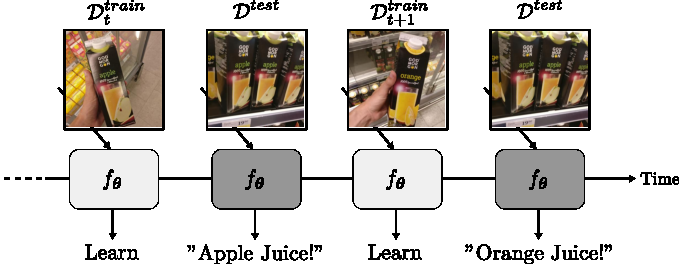
\includegraphics[width=0.8\textwidth]{Chapter4/imgs/cf_new.pdf}
	\caption{Illustration of catastrophic forgetting in a continual learning scenario. The network $f_{\vtheta}$ receives a task dataset of an Apple Juice class in $\gD_{t}^{train}$ to learn, and correctly predicts the Apple Juice class in the unseen test image in $\gD^{test}$. The next task dataset involves learning an Orange Juice class from $\gD_{t+1}^{train}$ which $f_{\vtheta}$ adapts to without retaining knowledge about the Apple Juice class, such that $f_{\vtheta}$ makes the wrong prediction during evaluation on $\gD^{test}$ again. }
	\vspace{-2mm}
	\label{fig:catastrophic_forgetting_example}
\end{figure}


\section{Related Work}\label{chap4:sec:related_work}

In this section, we give an overview of different approaches in CL, especially replay-based methods which our proposed replay scheduling approach in Paper \ref{paperC} and \ref{paperD} is based on. 

\vspace{-3mm}
\paragraph{Continual Learning.} The existing CL approaches for mitigating catastrophic forgetting in neural networks can broadly be divided into three main areas, namely, regularization-based, architecture-based, and replay-based methods. 
Regularization-based methods mainly focus on 
preventing the parameters important for previous tasks from wide changes and fit the remaining parameters to new tasks~\cite{kirkpatrick2017overcoming, zenke2017continual, nguyen2017variational}. 
Knowledge distillation methods~\cite{hinton2015distilling} also belong to these methods where stored classification logits are used for regularizing the output units for previous tasks in the network~\cite{li2017learning, schwarz2018progress}.
More recently, projection-based approaches have been proposed for constraining the parameter updates to subspaces which avoid interference with previous tasks~\cite{saha2021gradient, kao2021natural}. 
Architecture-based methods focus on adding task-specific network modules for every seen task~\cite{rusu2016progressive, yoon2017lifelong, yoon2019scalable, ebrahimi2020adversarial,xu2018reinforced}, or isolating parameters for predicting specific task in fixed-size networks~\cite{mallya2018packnet, serra2018overcoming, schwarz2021powerpropagation}. 
Replay-based methods revisits samples from old tasks when learning new tasks. The old samples are either stored in an external memory~\cite{chaudhry2019tiny, hayes2020remind, rolnick2018experience,jin2020gradient,verwimp2021rehearsal}, or synthesized with a generative model~\cite{shi2019variational, van2018generative, van2020brain, wu2018memory}. 
Both regularization- and architecture-based methods can be combined with replay for improving the models capability of remembering tasks~\cite{buzzega2020dark,douillard2020podnet,ebrahimi2020adversarial,joseph2020meta,mirzadeh2020linear,nguyen2017variational,pan2020continual,von2019continual}. 
Our replay scheduling idea is originated from replay-based methods which we will cover more in detail next. 

%\paragraph{Continual Learning.} There exist many different approaches in CL for mitigating catastrophic forgetting in neural networks. In general, these approaches can be divided into three main cores, namely, \textit{regularization-based}, \textit{architecture-based}, and \textit{replay-based} methods. Regularization-based methods are mainly focused on applying regularization techniques on parameters important for recognizing old tasks and fit the remaining parameters to new tasks~\cite{kirkpatrick2017overcoming, zenke2017continual, nguyen2017variational}. Knowledge distillation methods~\cite{hinton2015distilling} also belong to these approaches where classification logits are used for regularizing the output units for previous tasks in the network~\cite{li2017learning, schwarz2018progress}. More recently, there are some works that uses projection-based approaches for constraining the parameter updates to subspaces which avoid interference with previous tasks~\cite{saha2021gradient, kao2021natural}. Architecture-based approaches focuses on adding task-specific network modules for every seen task~\cite{rusu2016progressive, yoon2017lifelong, yoon2019scalable, ebrahimi2020adversarial}, or isolating parameters for predicting specific task in fixed-size networks~\cite{mallya2018packnet, serra2018overcoming, schwarz2021powerpropagation}. Replay-based methods re-trains on samples of old tasks when learning new tasks. The old samples are either stored in an external memory~\cite{chaudhry2019tiny, hayes2020remind, rolnick2018experience}, or synthesized with a generative model~\cite{shi2019variational, van2018generative, van2020brain, wu2018memory}. Both regularization- and architecture-based methods can be combined with replay for improving the models capability of remembering tasks [Add REFs]. Our replay scheduling idea is originated from replay-based methods which we will cover more in detail next. 

\vspace{-3mm}
\paragraph{Replay-based Continual Learning.} 
Much research effort in replay-based CL has focused on selecting higher quality samples to store in memory~\cite{aljundi2019gradient, borsos2020coresets, chaudhry2019tiny, chrysakis2020online, hayes2019memory, isele2018selective, lopez2017gradient, nguyen2017variational, rebuffi2017icarl, yoon2021online}. In \cite{chaudhry2019tiny}, several selection strategies are reviewed in scenarios with tiny memory capacity, such as reservoir sampling~\cite{vitter1985random}, first-in first-out buffer~\cite{lopez2017gradient}, k-Means, and Mean-of-Features~\cite{rebuffi2017icarl}. However, elaborate selection strategies have been shown to give little benefit over random selection for image classification problems~\cite{chaudhry2018riemannian, hayes2020remind}. 
More recent work has been focused on enhancing the memory capacity by storing compressed features rather than raw data~\cite{hayes2020remind, iscen2020memory, pellegrini2019latent}, evolving the memory samples using data augmentation to avoid overfitting~\cite{jin2020gradient,bang2021rainbow}, and using contrastive learning to improve memory retention~\cite{cha2021co2l,mai2021supervised}. 
Selecting the time to replay old tasks has mostly been ignored in the literature, with an exception in~\cite{aljundi2019online} which replays memory samples that would most interfere with a foreseen parameter update. Our replay scheduling approach differs from the above mentioned works since we focus on learning to select which tasks to replay. Nevertheless, our scheduling can be combined with any selection strategy and replay-based method.


%\paragraph{Replay-based Continual Learning.} In this thesis, we focus on replay-based methods with external memories for storing historical data. The most common selection strategy for filling the memory is random sampling from the used datasets. There exist several works focusing on selecting high quality samples for storing in the memory [Add REFs]. However, in image classification problems, random sampling has been shown to often perform on par with more elaborate selection strategies~\cite{chaudhry2018riemannian, hayes2020remind}. In contrast to using various memory selection methods, there has been proposals of retrieval policies over which samples to select for replay from the memory, for instance, selecting the samples that will mostly interfere with the parameter update with batches of new data~\cite{aljundi2019online}. Our replay scheduling approach differs from this method as we focus on selecting which tasks to select for replay rather than the individual samples to retrieve from the memory. More recent works have focused on evolving the memory samples through data augmentation to avoid overfitting to the memory [Add REFs], and also by using contrastive learning to improve discriminating between tasks. Another direction has been to increasing the storage capacity to store more samples by compressing raw data into features that are more memory-cheap [Add REFs]. The above mentioned methods assume that the memory is small and allocates equal storage amount for all tasks. Our new problem setting for memory-based CL is different from this assumption as we argue that data storage is cheap in many real-world applications. Hence, we compose a replay memory with data from historical tasks before learning new tasks because the amount of compute is limited. However, replay scheduling can be combined with of the mentioned methods as it only differs with the standard memory-based CL setting in that the replay memory has to be selected at every new task. 

%\vspace{-3mm}
%\paragraph{Generalization in Reinforcement Learning.} Generalization in RL is an active research field where much focus has been put on developing proper benchmark datasets for evaluating generalization capabilities of RL agents~\cite{cobbe2019quantifying, cobbe2020leveraging, nichol2018gotta, yu2020meta}.  Regularization techniques from supervised learning have been used to investigate whether these can enhance generalization in RL~\cite{cobbe2019quantifying, farebrother2018generalization, igl2019generalization}, and also how variations in the environments help to obtain agents that generalize better~\cite{packer2018assessing, zhang2018dissection}. Algorithms for enabling fast adaptation to new environments, such as new tasks~\cite{finn2017model, kessler2021same} and new action spaces~\cite{chandak2019learning, jain2020generalization}, has also been studied. The survey by Kirk \etal~\cite{kirk2021survey} focuses on zero-shot policy transfer where the policy must generalize to unseen dynamics in the test environments as additional queries could be disallowed in real-world scenarios~\cite{yang2019single, ball2021augmented}. In Paper \ref{paperD}, we consider using RL for learning policies for scheduling which tasks to replay in CL settings to mitigate catastrophic forgetting in the classifier. The policy is trained using experiences from multiple CL environments and then tested in new CL environments with unseen dynamics such as new task orders and datasets. 
%We evaluate our learned policies on the zero-shot policy transfer setting where the goal is to mitigate catastrophic forgetting in new CL scenarios. The rewards are accessible through accuracies calculated on validation datasets, however, fine-tuning the policy during CL training is prohibited.  



% General CL papers, add new papers that you have seen. Then Replay/memory-based CL approaches, add new and contrastive approaches. Perhaps something on meta-policy learning approaches, would be useful to tell how we use reinforcement learning here

%TO-DO \MK{A short and cozy table fo this, similar to survey by Delange etal 2021}
%\paragraph{Similarities and Differences between Continual Learning and other fields.} \MK{A short and cozy table fo this, similar to survey by Delange etal 2021}


\section{Replay Scheduling in Continual Learning}\label{chap4:sec:replay_scheduling_in_cl}

In this section, we present our proposed replay scheduling approach studied in Paper \ref{paperC} and \ref{paperD} for mitigating catastrophic forgetting in CL. 
More specifically, we focus on the contributions in Paper \ref{paperC}, where we introduce a slightly new CL setting that considers real-world needs where all historical data can be available since data storage is cheap. Additionally, we demonstrate the advantages of replay scheduling in such setting where we select which tasks to replay, where we use Monte Carlo tree search (MCTS)~\cite{coulom2006efficient} to search for efficient replay schedules by allowing multiple episodes in single CL environments. 


%In this section, we introduce a slightly new CL setting considering the real-world needs where all historical data can be available since data storage is cheap. However, the amount of compute is limited when the model is updated on new data due to operational costs. Hence, it is impossible for the model to leverage from all the available historical data to mitigate catastrophic forgetting. The goal then becomes to learn how we can select subsets of historical data for replay to efficiently reduce forgetting of the old tasks. We will refer to these subsets of historical data as the \textit{replay memory} throughout this chapter. The size of the replay memory affects the processing time when learning new tasks as well as the allowed time for the training phase. When composing the replay memory, we focus on determining the number of samples to draw from the seen tasks in the historical data rather than selecting single stored instances. Next, we introduce the problem setting in more detail as well as the notation of the new CL setting. 


\subsection{New Problem Setting for Continual Learning}

In this section, we describe the proposed CL setting presented in Paper \ref{paperC}. We assume that historical data is accessible at any time for mitigating catastrophic forgetting in the model. However, re-training the model on all available historical data is prohibited due to limitations on compute and data transmission times. Therefore, the goal is to determine which historical tasks to replay and sample a small replay memory from the selected tasks to mitigate catastrophic forgetting as efficiently as possible. 

The notation of this problem setting resembles the traditional CL setting for image classification. We let a neural network $f_{\vphi}$, parameterized by $\vphi$, learn $T$ tasks from the datasets $\gD_1, \dots, \gD_T$ arriving sequentially one at a time. The $t$-th dataset $\gD_t = \{(\vx_{t}^{(i)}, y_{t}^{(i)})\}_{i=1}^{N_{t}}$ consists of $N_t$ samples where $\vx_{t}^{(i)}$ and $y_{t}^{(i)}$ are the $i$-th data point and class label respectively. Additionally, the dataset is split into training, validation, and test sets such that $\gD_{1:T} = \{(\gD_{t}^{train}, \gD_{t}^{val}, \gD_{t}^{test})\}_{t=1}^{T}$. The training objective at task $t$ is given by 
%\vspace{-2mm}
\begin{align}
	\underset{\vphi}{\text{min}} \sum_{i=1}^{N_t} \gL(f_{\vphi}(\vx_t^{(i)}), y_{t}^{(i)}),
\end{align}
where $\gL(\cdot)$ is the loss function, which in our case is the cross-entropy loss. The challenge is for the network $f_{\vphi}$ to retain its classification performance on the previous $t-1$ tasks. 

We assume that historical data from old tasks are accessible at any time step. However, we can only fill a small replay memory $\gM$ with $M$ historical samples for mitigating catastrophic forgetting of old tasks due to processing time constraints. The challenge then becomes how to select the $M$ samples from the historical data to include in the replay memory that efficiently retain the previous knowledge. 
We focus on selecting the samples on task-level by deciding on the task proportions $(p_1, \dots, p_{t-1})$ on samples to fetch from each task, where $\sum_{i=1}^{t-1} p_i = 1$ and $p_{i} \geq 0$. The number of samples from task $i$ to place in $\gM$ is given by $p_i \cdot M$. To simplify the selection of which tasks to replay, we construct a finite set of possible task proportions that can be used for constructing $\gM$. 

This problem setting shares several assumptions with traditional CL, such as:
\begin{itemize}[noitemsep,topsep=1pt]
	\item The model receives the datasets at different time steps from a continuous stream.
	\item Re-training on all historical data is prohibited.
	\item The model should perform well overall across all seen tasks and, hence, mitigate catastrophic forgetting.
	\item Replay memory size $M$ is small.
\end{itemize}
The only difference with this setting and traditional CL is that all historical has been stored rather than deleted, and we can access this data to fill the replay memory $\gM$ to mitigate catastrophic forgetting. We argue that this setting aligns well with real-world needs as data storage is cheap and easy to maintain but retraining large machine learning models is computationally expensive. Therefore, we use small replay memory sizes to limit the processing times of replay when the model is learning new tasks. 


%\paragraph{Comparison to Traditional CL.} The new setting has several similarities to the traditional CL setting. Both settings share the fundamental setting that the data arrive in streams and re-training on all historical data is prohibited. Also, the goal that the model should perform well both historical tasks and tasks associated with new data remains the same. In replay-based CL, we also share the same constraints that the memory size is limited. However, we argue that this limitation is mainly associated with compute rather than of storage. Our assumption aligns with the real-world where data storage is cheap and easy to maintain, but retraining large machine learning models is computationally expensive. The only difference is that we allow filling the limited replay memory from historical data or some other external memory. Here, we argue that historical data is stored rather than deleted in many real-world settings~\cite{bailis2017macrobase}. Thus, we should keep the limited memory assumption for training but allow access to historical data to fill the replay memory to make CL align with real-world needs.
%\MK{TO-DO: this paragraph can be written in a more humble way, more like "this is something worth to investigate"}



%\subsection{Replay Scheduling for Mitigating Catastrophic Forgetting}
\subsection{Monte Carlo Tree Search for Replay Scheduling}

In this section, we describe how we used MCTS in Paper \ref{paperC} to show the advantages of replay scheduling in the new CL setting. We focus on an ideal CL environment where executing multiple episodes is allowed to enable searching for replay schedules. For demonstration purposes, we use MCTS for finding replay schedules that efficiently mitigate catastrophic forgetting by selecting compositions of replay memories at different time steps. 

\begin{wrapfigure}{r}{0.43\textwidth}
\hspace{-4mm}
\begin{minipage}{0.43\textwidth}
\vspace{-7mm}
\begin{algorithm}[H]
	\footnotesize
	\caption{Discretization of action space with task proportions}
	\label{alg:action_space_discretization}
	\begin{algorithmic}[1]
		\Require Number of tasks $T$
		\State $\gT = ()$ %\Comment{Initialize sequence for storing actions}
		\For{$i = 1, \dots, T-1$}
		\State $\gP_i = \{\}$ %\Comment{Set for storing task proportions at $i$}
		\State $\gB = \texttt{combinations}([1:i], i)$ %\Comment{Get bin vectors of size $i$ with bins $1, ..., i$}
		\State $\gB^{*} = \texttt{unique}(\texttt{sort}(\gB))$ %\Comment{Only keep unique bin vectors}
		\For{$\vb_i \in \gB^{*}$}
		\State $\vp_i = \texttt{bincount}(\vb_i) / i$ %\Comment{Calculate task proportion}
		\State $\gP_i = \gP_i \cup \{ \vp_i \}$ %\Comment{Add task proportion to set}
		\EndFor
		\State $\gT[i] = \gP_i$ %\Comment{Add set of task proportions to action sequence}
		\EndFor
		\State \Return $\gT$ %\Comment{Return action sequence as discrete action space}
	\end{algorithmic}
\end{algorithm}
\end{minipage}
\end{wrapfigure}
We define a replay schedule as a sequence $S = (\vp_1, \dots, \vp_{T-1})$, where $\vp_i = (p_1, \dots, p_{T-1})$ for $1 \leq i \leq T-1$ is the sequence of task proportions for determining how many samples per task to fill the replay memory with at time step $i$. 
To make the selection of task proportions tractable, we construct a discrete action space with a finite number of choices for how to construct the replay memory at different time steps. Algorithm \ref{alg:action_space_discretization} shows the procedure for creating this action space. At task $i$, we have $i-1$ historical tasks that we can choose from. We then generate all possible bin vectors $\vb_i = [b_1, \dots, b_{i}] \in \gB_i$ of size $i$ where each element are a task index $1, ..., i$. The elements in each bin vector are sorted by task index, and we only keep the unique bin vectors after sorting. For example, at $i=2$, the unique choices of vectors are $[1,1], [1,2], [2,2]$, where $[1,1]$ indicates that all samples in the replay memory should be from task 1, $[1,2]$ indicates that half memory is from task 1 and the other half are from task etc. 
The task proportions are then computed by counting the number of occurrences of each task index in $\vb_i$ and dividing by $i$, such that $\vp_i = \texttt{bincount}(\vb_i) / (i)$. From this specification, we have built a tree $\gT$ with different task proportions that can be selected at different time steps. A replay schedule $S$ is constructed by traversing through $\gT$ and appending a single task proportion from every task level to $S$.  


The tree-shaped action space of task proportions grows fast with the number of tasks, which complicates studying replay scheduling in datasets with longer task-horizons. 
Therefore, we proposed using MCTS since it has been successful in applications with large action spaces~\cite{browne2012survey, chaudhry2018feature, silver2016mastering}. In our case, MCTS concentrates the search for replay schedules in directions with promising CL performance in the environment. 
Each memory composition in the action space corresponds to a node that can be visited by MCTS. For instance, at task $t$, the node $v_t$ is related to a task proportions $\vp_{t}$ that can be used for retrieving a replay memory from the historical data. 
We store the related task proportion $\vp_t$ from every visited node $v_t$ in the replay schedule $S$. The final replay schedule is then used for constructing the replay memories at each task during the CL training. 
Figure \ref{fig:mcts_outline} shows an illustration of the procedure for executing MCTS to search for replay schedules, where each step involves the following:

\begin{figure}[t]
	\centering
	
\tikzstyle{block} = [rectangle, draw, %text width=4em, 
text centered, rounded corners, 
minimum width=6em,
minimum height=2em, node distance=3cm]
\tikzstyle{textblock} = [rectangle, text width=8em, 
text centered, font=\footnotesize\sffamily]
%minimum width=6em,
%minimum height=2em]
\tikzstyle{line} = [draw, -latex, very thick]
\tikzstyle{treenode} = [circle, draw, inner sep=2pt]
\tikzstyle{triangle} = [regular polygon,regular polygon sides=3, draw, inner sep=2pt]

\colorlet{myorange}{green!10!orange!90!}
\definecolor{midnightblue}{rgb}{0.1, 0.1, 0.44}
\definecolor{royalblue}{rgb}{0.25, 0.41, 0.88}

\begin{tikzpicture}[font=\small\sffamily]
	% Place nodes
	\node [block] (selection) {Selection}; 
	\node [block, right of=selection] (expansion) {Expansion};
	\node [block, right of=expansion] (simulation) {Simulation};
	\node [block, right of=simulation] (backprop) {Backpropagation};
	\node [rectangle, text centered, above of=expansion, xshift=4em, yshift=-0.8em] (repeat) {Repeat X times};
	\node [textblock, below of=selection, yshift=-6em] (test) {Execute tree policy until a leaf node at task $t$ is reached};
	\node [textblock, below of=expansion, yshift=-6em] (test) {Create new node in tree at task $t+1$};
	\node [textblock, below of=backprop, yshift=-6.5em] (test) {The result from replay schedule is backpropagated through the tree};
	% Draw edges
	\path [line] (selection) -- (expansion);
	\path [line] (expansion) -- (simulation);
	\path [line] (simulation) -- (backprop);
	\path [line] (repeat.west) -- ($(repeat.west) - (13.3em,0)$) |- (selection.west);
	\path [line, -] (backprop.east) -- ($(backprop.east) + (0.5em,0)$) |- (repeat.east);
	
	% Place trees
	% Selection tree
	\node [treenode, below of=selection, very thick, royalblue, yshift=1em] {} [sibling distance=1.5em, level distance=1.5em] {} 
	child[very thick, royalblue, ->] { node [treenode] {}
		child[thin, black, -] { node [treenode] {} }
		child[very thick, royalblue] { node [treenode] {}
		}
	}
	child { node [treenode] {}}
	child { node [treenode] {}
		child { node [treenode] {}}
		child { node [treenode] {}}
	};
	% Expansion tree
	\node [treenode, below of=expansion, yshift=1em] {} [sibling distance=1.5em, level distance=1.5em] {} 
	child[] { node [treenode] {}
		child[] { node [treenode] {}}
		child[] { node [treenode, very thick, royalblue] {}
			child[very thick, royalblue, ->] { node [treenode] {}} }}
	child { node [treenode] {}}
	child { node [treenode] {}
		child { node [treenode] {}}
		child { node [treenode] {}}};
	% Simulation tree
	\node [treenode, below of=simulation, yshift=1em] {} [sibling distance=1.5em, level distance=1.5em] {} 
	child[] { node [treenode] {}
		child[] { node [treenode] {}}
		child[] { node [treenode] {}
			child[] { node [treenode, very thick, royalblue] {}
				child[very thick, dashed, royalblue, ->] { node [triangle, yshift=-3em, solid] {} edge from parent node [right, black, text width=5em, font=\footnotesize\sffamily, xshift=0.4em] {Simulation until task $T$ is reached}}
			} 
		}
	}
	child { node [treenode] {}}
	child { node [treenode] {}
		child { node [treenode] {}}
		child { node [treenode] {}}};
	% Backprop tree    
	\node [treenode, below of=backprop, very thick, myorange, yshift=1em] {} [sibling distance=1.5em, level distance=1.5em] {} 
	child[very thick, myorange, <-]  { node [treenode] {}
		child[thin, black, -] { node [treenode] {}}
		child[very thick, myorange, <-]  { node [treenode] {}
			child[very thick, myorange, <-] { node [treenode] {}} }}
	child { node [treenode] {}}
	child { node [treenode] {}
		child { node [treenode] {}}
		child { node [treenode] {}}
	};
	
\end{tikzpicture}
	\caption{Outline of MCTS when searching for replay schedules. }
	\label{fig:mcts_outline}
	\vspace{-2mm}
\end{figure}

\begin{itemize}[topsep=1pt, itemsep=1pt, label={}, leftmargin=*]
	\item {\bf Selection.} During a rollout, the tree policy either selects an unvisited child randomly from the current node $v_t$, or selects the next node by evaluating the Upper Confidence Tree (UCT)~\cite{kocsis2006bandit} if all children has been visited earlier.
	The child $v_{t+1}$ with the highest UCT score is selected using the function from \cite{chaudhry2018feature}:
	\begin{align}\label{eq:uct}
		UCT(v_t, v_{t+1}) = \text{max}(q(v_{t+1})) + C \sqrt{\frac{2 \log(n(v_{t}))}{n(v_{t+1})}},
	\end{align}
	where $q(\cdot)$ is the reward function, $C$ the exploration constant, and $n(\cdot)$ the number of node visits. The tree policy is executed until a leaf node $v_t$ is reached.
	
	\item {\bf Expansion.} If the leaf node $v_t$ has unvisited children, the search tree is expanded with one of the unvisited child nodes $v_{t+1}$ selected with uniform sampling. 
	
	\item {\bf Simulation and Reward.} After the expansion step, the succeeding nodes are selected randomly until reaching a terminal node $v_T$. The task proportions $\vp_{1:T-1}$ from the visited nodes in the rollout constitutes the replay schedule $S$. After training the network using $S$ for replay, we calculate the reward for the rollout given by $r = \frac{1}{T} \sum_{i=1}^T A_{T, i}^{(val)}$, where $A_{T, i}^{(val)}$ is the validation accuracy of task $i$ at task $T$.  
	
	\item {\bf Backpropagation.} The reward $r$ is backpropagated from the expanded node $v_{t+1}$ to the root node, where the reward function $q(\cdot)$ and number of visits $n(\cdot)$ are updated at each node in the path. 
\end{itemize}
As mentioned earlier, we use MCTS to search for replay schedules to illustrate the importance of learning the time to learn. To this end, we study replay scheduling in an ideal CL environment where multiple episodes is allowed to find replay schedules. However, in the standard CL setting, multiple episodes are prohibited which currently prevents replay scheduling to be applied in real-world CL scenarios. In the next section, we present a policy learning framework based on RL to learn replay scheduling policies that generalize. 


%\section{Meta Policy Learning for Replay Scheduling}\label{sec:meta_policy_learning_for_replay_scheduling}
\section{Policy Learning for Replay Scheduling}\label{chap4:sec:policy_learning_for_replay_scheduling}

In this section, we introduce the RL-based framework for learning replay scheduling policies that was proposed in Paper \ref{paperD}. In real-world CL settings, learning the policy with multiple episodes is infeasible, which is why we need a general policy for replay scheduling.
Our intuition is that there may exist general patterns regarding the replay scheduling, e.g., tasks that are harder or have been forgotten should be replayed more often. Moreover, the policy may non-trivially take task properties into consideration. Therefore, we aim to learn policies that select which tasks to replay from states representing the current task performance in the CL environments. The policy can then be applied for mitigating catastrophic forgetting in new CL scenarios. 

We model the CL environments as Markov Decision Processes~\cite{bellman1957markovian} (MDPs) where each MDP is represented as a tuple $E_i = (\gS_i, \gA, P_i, R_i, \mu_i, \gamma)$ consisting of the state space $\gS_i$, action space $\gA$, state transition probability $P_i(s' | s, a)$, reward function $R_i(s, a)$, initial state distribution $\mu_i(s_1)$, and discount factor $\gamma$.
We assume that we have access to a fixed set of training environments $\gE^{(train)} = \{E_1, \dots, E_K\}$ sampled from a distribution of CL environments, i.e., $E_i \sim p(E)$ for $i=1, ..., K$. 
Each environment $E_i$ contains of a network $f_{\vphi}$ and $T$ datasets $\gD_{1:T}$ where the $t$-th dataset is learned by $f_{\vphi}$ at time step $t$. Note that we will use task and time step interchangeably. 
To generate diverse CL environments, we obtain environments with different initializations of the network $f_{\vphi}$ and shuffled task orders in the dataset when we sample environments from $p(E)$. 

We define the state $s_t$ of the environment as the validation accuracies $A_{t, 1:t}^{(val)}$ on each seen task $1, ..., t$ from $f_{\vphi}$ at task $t$, i.e., $s_t = [A_{t, 1}, ..., A_{t, t}, 0, ..., 0]$, where we use zero-padding on future tasks. The action space $\gA$ is constructed as described in Algorithm \ref{alg:action_space_discretization} (Section \ref{chap4:sec:replay_scheduling_in_cl}), such that the $a_t \in \gA$ corresponds to a task proportion $\vp_t$ used for sampling the replay memory $\gM_t$. We use a dense reward based on the average validation accuracies at task $t$, i.e., $r_{t} = \frac{1}{t}\sum_{i=1}^{t} A_{t, i}^{(val)}$. The state transition distribution $P_i(s' | s, a)$ represents the dynamics of the environment, which depend on the initialization of $f_{\vphi}$ and also the task order in the dataset. More specifically, the dynamics represent how the validation accuracies varies after $f_{\vphi}$ replays according to the action $a_t$ when learning the current task. 

The procedure for training the policy goes as follows: 
The state $s_t$ is obtained by evaluating the network $f_{\vphi}$ on the validation sets $\gD_{1:t}^{(val)}$ after learning the $t$-th task from $\gD_t^{(train)}$. Action $a_t$ is selected under the policy $\pi_{\vtheta}(a | s_t)$ parameterized by $\vtheta$. The action is converted into task proportion $\vp_t$ that is used for sampling the replay memory $\gM_t$ from the historical datasets. 
We then train classifier $f_{\vphi}$ with $\gD_{t+1}^{(train)}$ and $\gM_t$, and obtain the reward $r_{t+1}$ and the next state $s_{t+1}$ by evaluating $f_{\vphi}$ on the validation sets $\gD_{1:t+1}^{(val)}$. The collected transitions $(s_t, a_t, r_{t+1}, s_{t+1})$ are used for updating the policy.  A new episode starts after $f_{\vphi}$ has learned the final task $T$. 

We evaluate the learned policy by applying it to mitigate catastrophic forgetting in new CL environments at test time. To foster generalization across environments, we train the policy on multiple environments with different dynamics, such as task orders and datasets, to learn from a diverse set of training data. The goal for the agent is to maximize the sum of rewards in each training environment. 
At test time, the policy is applied on new CL classifiers and datasets in the test environments without added computational cost nor experience collection. In Section \ref{chap4:sec:experiments}, we test the policies generalization capability to new CL environments where the task orders and datasets are unseen during training.


%In this section, we present an RL-based framework to learn policies for selecting which tasks to replay in CL scenarios. We are interested in learning such policy that can be transferred to new CL scenarios, such as new task orders and new datasets, without any additional computational cost for updating on the new domain. We take a meta-learning approach where the policy learns from episodes of experience collected from training a classifier in CL settings. The experience from the environment is represented as the classification performance on each seen task in the dataset. The policy receives the task performances for basing its action on which task that needs to be replayed at the next time step. Our goal is to obtain a policy that can generalize to be used for replay scheduling in new CL scenarios to mitigate catastrophic forgetting. Next, we describe in more detail how the framework for learning this policy works.

%By learning from gathering experience, the policy learns better for the future on how to select the tasks to replay. However, as 

%\MK{Is this how it should be motivated?}
%Imagine the scenario that we can collect experiences from many users applying their phone to CL scenarios for learning different objects to recognize sequentially. Assume that we can store the collected data (limitation here is privacy!), the models will suffer from catastrophic forgetting as they are trained in CL scenario. But we can then use the collected data to train a replay scheduling policy. The learned policy can then be transferred to new users using their phone in CL settings and the policy is used for mitigating catastrophic forgetting in their environment without additional computational cost. 

%Limitations here are of course that we potentially need lots of data for learning a policy that generalizes. Additionally, we need lots of training time and hyperparameter tuning as we are dealing with RL. Also, we need to store the data somewhere which is cheap, but it must be secure due to privacy concerns. An alternative there could be to store features instead of raw data, which is not completely flawless (I think that it's possible to revert features back to the real data to some extent) but at least it is a safer alternative. Another option for the data needed can be to gather experience from simulated environments and benchmark datasets. As the policy only takes in states with task performances, we can make use mixes of benchmark datasets and data from real contributing users. 

\begin{comment}
	
\subsection{Problem Setting}

We consider the setting where an agent selects replay schedules to mitigate catastrophic forgetting in a classifier trained in the CL setting. The environment that the agent interacts with contains a network $f_{\vphi}$ and a dataset $\gD_{1:T}$ of $T$ tasks that $f_{\vphi}$ should learn in sequential order. The dataset is split into training, validation, and test sets as $\gD_{1:T} = \{\gD_{1:T}^{\train}, \gD_{1:T}^{\val}, \gD_{1:T}^{\test}\}$ respectively. The training sets $\gD_{1:T}^{\train}$ are for the network to learn all $T$ tasks sequentially, while the $\gD_{1:T}^{\val}$ are for evaluating how well the network performs on each task during training. The task performances on the validation sets can be used for dense rewards to the RL agent. The test sets are for final evaluation and are unseen during training as standard practice to avoid overfitting.  

We consider having a distribution $p(E)$ of Markov Decision Process~\cite{bellman1957markovian} (MDP) where the MDP is represented as a tuple $E_i = (\gS_i, \gA, P_i, R_i, \mu_i, \gamma)$ consisting of the state space $\gS_i$, action space $\gA$, state transition probability $P_i(s' | s, a)$, reward function $R_i(s, a)$, initial state distribution $\mu_i(s_0)$, and discount factor $\gamma$. For training, we assume that we have access to a fixed set of training environments $\gE_{\train} = \{E_1, \dots, E_K\}$, where $E_i \sim p(E)$ for $i=1, ..., K$. Each environment $E_i$ contains of a network $f_{\vphi}$ and $T$ datasets $\gD_{1:T}$ where the $t$-th dataset is learned at time step $t$. We let the dynamics of the environments depend on the network initialization and the task order of the datasets. The states $s$ are given by the validation performance on each task from $f_{\vphi}$ which can be accuracies. Hence, the state space $\gS_i$ depends on the parameter initialization for $\vphi$. Regarding the datasets, we allow the task orders in the datasets $\gD_{1:T}$ to be shuffled for each sampled environment $E_i \sim p(E)$. Therefore, the state space is also affected by the task order as this can yield different CL performances. We assume that the action space is the same for every environment as the agent will interact with each training environment in $\gE_{\train}$. 

The goal for the agent is to maximize the accumulated returns in each training environment. The reward is given by the CL performance. We assume that we have a dense reward that we can compute from the validation sets at each time step $t$. We are therefore after a policy that works well on all environments. The intention for learning such policy is that it should generalize across environments of new CL settings, such as new task orders and datasets. As we are not allowed to go back in time in CL, we are not allowed to query the testing environments during the transfer. Hence we must apply the policy in a zero-shot setting where tuning the policy on the testing environment is prohibited.


\subsection{Deep Q-Networks for Learning Replay Scheduling Policy}

We employ DQNs for learning the policy for replay scheduling. The architecture takes states as input and outputs action values for the valid actions at the current time step $t$. We define the states $s$ as a vector with the validation performance of every seen task, where we use the validation accuracy to represent the task performance. We use zero-padding on the vector elements in the states that represent the performance for future tasks. The states can also be represented by other performance metrics, for example, the accuracy difference between time steps or forgetting measures such as backward transfer~\cite{lopez2017gradient} (BWT). For the actions, we use the discrete action space built using Algorithm \ref{alg:action_space_discretization} such that the action space $\gA_t$ is time-dependent and grows per seen task. To handle the growing action space, we assume that we know the total number of actions such that the DQN can use a fixed output layer. Therefore, we use action masking on the predicted action values to prevent the DQN from selecting invalid actions. 

\begin{algorithm}[t]
	\caption{Learning replay scheduling policy with DQN}
	\label{alg:learning_replay_scheduling_policy_with_dqn}
	\begin{algorithmic}[1]
		\Require $\gE_{\train}$: Training environments
		\Require $\vtheta$: DQN parameters
		\State $\gB = \{\}$ \Comment{Initialize replay buffer}
		\For{$i = 1, \dots, n_{\text{episodes}}$}
		\State $s_1^{i} \sim \mu_i \, \forall E_i \in \gE_{\train}$ \Comment{Get initial states}
		\For{$t=1, \dots, T-1$}
		\For{$E_i \in \gE_{\train}$}
		\State $a_t^{i} = \argmax_{a' \in \gA_t} Q_{\vtheta}(s_t^{i}, a')$ \Comment{Get actions from states}
		\State $r_t^{i}, s_{t+1}^{i} = \texttt{CLStep}(t, a_t^{i}, E_i)$
		\State $\gB = \gB \cup \{(s_{t}^{i}, a_{t}^{i}, r_{t}^{i}, s_{t+1}^{i})\}$ \Comment{Store transition in buffer}
		\State $(s_j, a_j, r_j, s_{j+1}) \stackrel{B}{\sim} \gB$ \Comment{Get mini-batch of $B$ samples from buffer}					
		%\State $\{(s_t^{(j)}, a_t^{(j)}, r_t^{(j)}, s_{t+1}^{(j)})\}_{j=1}^{B} \stackrel{B}{\sim} \gB$
		\State $\vtheta \leftarrow \vtheta - \eta \nabla_{\vtheta} (r_t + \max_{a'} Q_{\vtheta^{-}}(s_{j+1}, a') - Q_{\vtheta}(s_j, a_j))$ \Comment{Update DQN}
		\EndFor
		\EndFor 
		\EndFor
		\State \Return $\vtheta$ \Comment{Return DQN}
		
		\Statex
		
		\Function{\texttt{CLStep}}{$t$, $a_{t}$, $E$}
		\State $\gM_t \leftarrow \texttt{SampleMemory}(a_t)$ \Comment{Sample historical data from action}
		\State $f_{\vphi}^{E} \leftarrow \texttt{Train}(f_{\vphi}^{E}, \gD_{t+1}^{\train}, \gM_t)$ \Comment{Train network on current task with replay}
		\State $r_t \leftarrow \frac{1}{t+1} \sum_{i=1}^{t+1} A_{i}^{\val}$ \Comment{Compute reward from validation datasets}
		\State $s_{t+1} \leftarrow \texttt{GetState}(f_{\vphi}^{E}, \gD_{1:t+1}^{\val})$ \Comment{Get next state from validation performance}
		\State \Return $r_t$, $s_{t+1}$ \Comment{Return reward and next state}
		\EndFunction
	\end{algorithmic}
\end{algorithm}

We outline the procedure for training the DQN on multiple CL environments in Algorithm \ref{alg:learning_replay_scheduling_policy_with_dqn}. The main idea to obtain a policy that generalize is to train it on several environments with different dynamics for learning from more diverse training data~\cite{zhang2018dissection}. We let the DQN store transitions $(s_{t}^{i}, a_{t}^{i}, r_{t}^{i}, s_{t+1}^{i})$ from all environments in the same experience replay buffer $\gB$ to use for training the network. The first step is to receive the intial state $s_1$ for all environments by training the network $f_{\vphi}$ on the first dataset $\gD_1^{\train}$ in each environment, such that $s_{1}^{i} = [A_{1,1}^{\val}, 0, ..., 0]$. The DQN then selects the action $a_t$ for the current environment from the input state or selects a random action with probability $\epsilon$. The agent retrieves the reward and next state by training the environment-specific network $f_{\vphi}^{i}$ on the current task $t$ in \texttt{CLStep}. Before training starts, the action $a_{t}^{i}$ is used for sampling the replay memory $\gM_t$ using the task proportions $(\vp_1, \dots, \vp_{T-1})$ translated from $a_{t}^{i}$. The replay memory is then used for mitigating catastrophic forgetting when training on the current task. After training, the agent obtains the reward from the reward function 
\begin{align}
	R(s, a) = \frac{1}{t} \sum_{i=1}^{t} A_{t, i}^{\val},
\end{align}
where $A_{t, i}^{\val}$ is the validation accuracy on task $i$ after $f_{\vphi}$ has learned task $t$. The next state is also obtained by utilizing the validation accuracies up to task $t$, such as $s_{t+1}^{i} = [A_{t, 1}^{\val}, ..., A_{t, t}^{\val}, 0, ..., 0] \in [0, 1]^{T-1}$. The DQN is then updated by sampling a mini-batch of $B$ samples from the shared buffer $\gB$ and taking a gradient step to minimize the loss
\begin{align}
	\gL_{\text{DQN}}(\vtheta) = r_j + \max_{a'} Q_{\vtheta^{-}}(s_{j+1}, a') - Q_{\vtheta}(s_j, a_j), 
\end{align}  
where $\vtheta^{-}$ is target network which is copy of the parameters $\vtheta$ from some previous time step. By using the shared replay buffer, the DQN is trained on diverse set of environments that can generalize well to new environments with unseen dynamics from an unseen task order or a new dataset. Next, we will describe the experiments we perform to evaluate the generalization capability of the policy to new CL scenarios. 
\end{comment}


\section{Experiments}\label{chap4:sec:experiments}

In this section, we give an overview of the experimental results from Paper \ref{paperC} and \ref{paperD}. In Paper \ref{paperC}, we evaluate the benefits of replay scheduling in single CL environments using MCTS for finding replay schedules. We perform extensive evaluation to show that the replay schedules from MCTS can outperform the baselines across several CL benchmarks and different backbones. 
In Paper \ref{paperD}, we evaluate our RL-based framework using DQN~\cite{mnih2013playing} and A2C~\cite{mnih2016asynchronous} for learning policies that generalize to new CL scenarios.
We show that the learned policies can efficiently mitigate catastrophic forgetting in CL environments with new task orders and datasets that are unseen during training. 
%Full details on experimental settings and additional results are in Appendix \ref{app:experimental_settings} and \ref{app:additional_experimental_results}. Code is available as supplementary material.  

%In this section, we give an overview of the experimental results in Paper \ref{paperC} and \ref{paperD}. In Paper \ref{paperC}, we perform experiments to show that the importance of replay scheduling in our proposed problem setting for CL described in Section \ref{sec:replay_scheduling_in_cl}. We demonstrate that learning when to replay different tasks by using MCTS as an exemplar method for finding good replay schedules that are efficient in mitigating catastrophic forgetting in the classifier. In Paper \ref{paperD}, we demonstrate on benchmark datasets for CL how our RL-based framework can be used for learning replay scheduling policies. We show that our proposed method can learn policies that generalize to CL scenarios with new task orders and datasets unseen during training.  

\subsection{Results on Replay Scheduling with Monte Carlo Tree Search}

Here, we provide a selection of the experimental results from Paper \ref{paperC}. Our approach has been named Replay Scheduling MCTS (RS-MCTS). 
We evaluate the CL performance of RS-MCTS for varying memory sizes to illustrate the importance of replay scheduling. Moreover, we show that replay scheduling can benefit any replay-based method by combining scheduling with three recent CL methods, namely, HAL~\cite{chaudhry2021using}, MER~\cite{riemer2018learning}, and DER~\cite{buzzega2020dark}. Finally, we demonstrate the efficiency benefits of replay scheduling in settings when the memory size is smaller than the number of classes. We give an overview of the experimental settings, see Paper \ref{paperC} for the full experimental results and hyperparameter settings. 

\vspace{-3mm}
\paragraph{Datasets and Architectures.} We perform experiments on common CL benchmark datasets such as Split MNIST~\cite{zenke2017continual}, Split Fashion-MNIST~\cite{xiao2017fashion}, Split notMNIST~\cite{bulatov2011notMNIST}, Permuted MNIST~\cite{goodfellow2013empirical}, and Split CIFAR-100~\cite{krizhevsky2009learning, lopez2017gradient, rebuffi2017icarl} and Split miniImagenet~\cite{vinyals2016matching}. We use a 2-layer MLP with 256 hidden units and ReLU activations for Split MNIST, Split FashionMNIST, Split notMNIST, and Permuted MNIST.  For Split CIFAR-10 and CIFAR-100, we use the CNN architecture used in \cite{adel2019continual, schwarz2018progress, vinyals2016matching}, and a reduced ResNet-18 from \cite{lopez2017gradient} for Split mini-Imagenet. We use a multi-head output layer for each dataset, except Permuted MNIST where the network uses single-head output layer, such that we assume that task labels are available at test time~\cite{van2019three}. 

\vspace{-3mm}
\paragraph{Baselines.} We compare our method against the following scheduling baselines:
\begin{itemize}[itemsep=0em,topsep=1pt]
	\item {\bf Random Schedule}: Randomly select which tasks to replay.
	\item {\bf Equal Task Schedule (ETS)}: Replay all seen tasks equally.
	\item {\bf Heuristic Schedule}: Replay tasks which validation performance is below a tuned threshold found through hyperparameter searches.
\end{itemize} 

\vspace{-3mm}
\paragraph{Evaluation.} We use the following evaluation metric for measuring the CL performance
\begin{align}\label{eq:acc}
	\ACC = \frac{1}{T} \sum_{j=1}^{T} A_{T, j}^{test},
\end{align}
where $A_{T, j}^{test}$ is the accuracy of task $j$ after learning the final task $T$.  
%In Paper \ref{paperD}, we use a ranking method for comparing the ACC performance of each scheduling method within the testing environments, since the performance between environments can differ significantly when the task order changes. We then average all obtained ranking lists over the number of testing environments to obtain the ranking metric. 

\vspace{-3mm}
\begin{wrapfigure}{r}{0.50\textwidth}
	%\centering
	\vspace{-3mm}
	\hspace{-11mm}
	%\begin{minipage}{0.50\textwidth}
	\setlength{\figwidth}{0.36\textwidth}
	\setlength{\figheight}{.16\textheight}
	\resizebox{0.58\textwidth}{!}{
		


\pgfplotsset{every axis title/.append style={at={(0.5,0.80)}}} 
\pgfplotsset{every tick label/.append style={font=\tiny}}
\pgfplotsset{every major tick/.append style={major tick length=2pt}}
\pgfplotsset{every minor tick/.append style={minor tick length=1pt}}
\pgfplotsset{every axis x label/.append style={at={(0.5,-0.22)}}}
\pgfplotsset{every axis y label/.append style={at={(-0.17,0.5)}}}
´

\begin{tikzpicture}
\tikzstyle{every node}=[font=\scriptsize]
\definecolor{color0}{rgb}{0.12156862745098,0.466666666666667,0.705882352941177}
\definecolor{color1}{rgb}{1,0.498039215686275,0.0549019607843137}
\definecolor{color2}{rgb}{0.172549019607843,0.627450980392157,0.172549019607843}
\definecolor{color3}{rgb}{0.83921568627451,0.152941176470588,0.156862745098039}

\begin{groupplot}[group style={group size= 2 by 2, horizontal sep=0.7cm, vertical sep=0.8cm}]

\nextgroupplot[title=Split MNIST,
height=\figheight,
legend cell align={left},
legend columns=4,
legend style={
  nodes={scale=0.80},
  fill opacity=0.8,
  draw opacity=1,
  text opacity=1,
  at={(0.00,1.30)}, %{(3.70,-0.30)},   %{(3.72,0.13)},
  anchor=south west,
  draw=white!80!black
},
minor xtick={},
minor ytick={},
tick align=outside,
tick pos=left,
width=\figwidth,
x grid style={white!69.0196078431373!black},
xmajorgrids,
%xlabel={Memory size \(\displaystyle M\)},
xmin=0.7, xmax=7.3,
xtick style={color=black},
xtick={1,2,3,4,5,6,7},
xticklabels={8,24,80,120,200,400,800},
y grid style={white!69.0196078431373!black},
ymajorgrids,
ylabel={ACC (\%)},
ymin=0.939, ymax=0.997729043511215,
ytick style={color=black},
ytick={0.92,0.93,0.94,0.95,0.96,0.97,0.98,0.99,1},
yticklabels={92,93,94,95,96,97,98,99,100}
]
\path [fill=color0, fill opacity=0.2, line width=1pt]
(axis cs:1,0.92504620552063)
--(axis cs:1,0.981783270835876)
--(axis cs:2,0.981537520885468)
--(axis cs:3,0.988991677761078)
--(axis cs:4,0.986135482788086)
--(axis cs:5,0.991755723953247)
--(axis cs:6,0.989374697208405)
--(axis cs:7,0.994002878665924)
--(axis cs:7,0.976767957210541)
--(axis cs:7,0.976767957210541)
--(axis cs:6,0.979170620441437)
--(axis cs:5,0.964531421661377)
--(axis cs:4,0.978874921798706)
--(axis cs:3,0.979120314121246)
--(axis cs:2,0.937642157077789)
--(axis cs:1,0.92504620552063)
--cycle;

\path [fill=color1, fill opacity=0.2, line width=1pt]
(axis cs:1,0.946015386753438)
--(axis cs:1,0.970621573246562)
--(axis cs:2,0.984533286206628)
--(axis cs:3,0.988692537329328)
--(axis cs:4,0.990023216819651)
--(axis cs:5,0.990669279851693)
--(axis cs:6,0.992800317892538)
--(axis cs:7,0.994021984494329)
--(axis cs:7,0.992872175505671)
--(axis cs:7,0.992872175505671)
--(axis cs:6,0.990845362107462)
--(axis cs:5,0.986030240148307)
--(axis cs:4,0.986402863180349)
--(axis cs:3,0.980789062670673)
--(axis cs:2,0.972900553793372)
--(axis cs:1,0.946015386753438)
--cycle;

\path [fill=color2, fill opacity=0.2, line width=1pt]
(axis cs:1,0.953295697386423)
--(axis cs:1,0.969893182613577)
--(axis cs:2,0.989900327489411)
--(axis cs:3,0.987615676138068)
--(axis cs:4,0.987468694435405)
--(axis cs:5,0.987904186526891)
--(axis cs:6,0.990390603540462)
--(axis cs:7,0.991611458769248)
--(axis cs:7,0.983504221230752)
--(axis cs:7,0.983504221230752)
--(axis cs:6,0.978347876459538)
--(axis cs:5,0.975166293473109)
--(axis cs:4,0.979932985564595)
--(axis cs:3,0.979642883861932)
--(axis cs:2,0.966454952510589)
--(axis cs:1,0.953295697386423)
--cycle;

\path [fill=color3, fill opacity=0.2, line width=1pt]
(axis cs:1,0.976848125457764)
--(axis cs:1,0.986456036567688)
--(axis cs:2,0.988981068134308)
--(axis cs:3,0.992213249206543)
--(axis cs:4,0.991635799407959)
--(axis cs:5,0.991742670536041)
--(axis cs:6,0.992980241775513)
--(axis cs:7,0.994612276554108)
--(axis cs:7,0.993073880672455)
--(axis cs:7,0.993073880672455)
--(axis cs:6,0.992027640342712)
--(axis cs:5,0.990043103694916)
--(axis cs:4,0.989341855049133)
--(axis cs:3,0.989036798477173)
--(axis cs:2,0.982677280902863)
--(axis cs:1,0.976848125457764)
--cycle;

\addplot [line width=1.0pt, color0, mark=*, mark size=1, mark options={solid}]
table {%
1 0.953414738178253
2 0.959589838981628
3 0.984055995941162
4 0.982505202293396
5 0.978143572807312
6 0.984272658824921
7 0.985385417938232
};
\addlegendentry{Random}
\addplot [line width=1.0pt, color1, mark=*, mark size=1, mark options={solid}]
table {%
1 0.95831848
2 0.97871692
3 0.9847408
4 0.98821304
5 0.98834976
6 0.99182284
7 0.99344708
};\addlegendentry{ETS}
\addplot [line width=1.0pt, color2, mark=*, mark size=1, mark options={solid}]
table {%
1 0.96159444
2 0.97817764
3 0.98362928
4 0.98370084
5 0.98153524
6 0.98436924
7 0.98755784
};
\addlegendentry{Heuristic}
\addplot [line width=1.0pt, color3, mark=*, mark size=1, mark options={solid}]
table {%
1 0.981652081012726
2 0.985829174518585
3 0.990625023841858
4 0.990488827228546
5 0.990892887115479
6 0.992503941059113
7 0.993843078613281
};\addlegendentry{Ours}




%
\nextgroupplot[title=Split FashionMNIST,
height=\figheight,
legend cell align={left},
legend style={
  nodes={scale=0.7},
  fill opacity=0.8,
  draw opacity=1,
  text opacity=1,
  at={(0.48,0.03)},
  anchor=south west,
  draw=white!80!black
},
minor xtick={},
minor ytick={0.89, 0.91, 0.93, 0.95, 0.97, 0.99},
tick align=outside,
tick pos=left,
width=\figwidth,
x grid style={white!69.0196078431373!black},
xmajorgrids,
%xlabel={Memory size \(\displaystyle M\)},
xmin=0.7, xmax=7.3,
xtick style={color=black},
xtick={1,2,3,4,5,6,7},
xticklabels={8,24,80,120,200,400,800},
y grid style={white!69.0196078431373!black},
ymajorgrids,
yminorgrids,
%ylabel={ACC},
ymin=0.899,%0.891766529814355,
ymax=0.996494715797058,
ytick style={color=black},
ytick={0.88,0.9,0.92,0.94,0.96,0.98,1},
yticklabels={88, 90, 92, 94, 96, 98, 100}
]
\path [fill=color0, fill opacity=0.2, line width=1pt]
(axis cs:1,0.96419358253479)
--(axis cs:1,0.976246356964111)
--(axis cs:2,0.984048008918762)
--(axis cs:3,0.98274040222168)
--(axis cs:4,0.982234418392181)
--(axis cs:5,0.985867142677307)
--(axis cs:6,0.985980749130249)
--(axis cs:7,0.988571465015411)
--(axis cs:7,0.980668723583221)
--(axis cs:7,0.980668723583221)
--(axis cs:6,0.972739219665527)
--(axis cs:5,0.975212812423706)
--(axis cs:4,0.954325616359711)
--(axis cs:3,0.976219773292542)
--(axis cs:2,0.962551951408386)
--(axis cs:1,0.96419358253479)
--cycle;

\path [fill=color1, fill opacity=0.2, line width=1pt]
(axis cs:1,0.965724160568608)
--(axis cs:1,0.979275839431391)
--(axis cs:2,0.983843648420532)
--(axis cs:3,0.987767732323772)
--(axis cs:4,0.988072744085454)
--(axis cs:5,0.988506841180757)
--(axis cs:6,0.989178836422143)
--(axis cs:7,0.990307375485654)
--(axis cs:7,0.989052624514346)
--(axis cs:7,0.989052624514346)
--(axis cs:6,0.987461163577857)
--(axis cs:5,0.983413158819243)
--(axis cs:4,0.982567255914546)
--(axis cs:3,0.970792267676228)
--(axis cs:2,0.972876351579468)
--(axis cs:1,0.965724160568608)
--cycle;

\path [fill=color2, fill opacity=0.2, line width=1pt]
(axis cs:1,0.955000050761585)
--(axis cs:1,0.970759949238415)
--(axis cs:2,0.98603178628668)
--(axis cs:3,0.981832320290786)
--(axis cs:4,0.983967730086771)
--(axis cs:5,0.978253058795492)
--(axis cs:6,0.991734343706935)
--(axis cs:7,0.969833098095523)
--(axis cs:7,0.896526901904478)
--(axis cs:7,0.896526901904478)
--(axis cs:6,0.916425656293065)
--(axis cs:5,0.938266941204508)
--(axis cs:4,0.921192269913229)
--(axis cs:3,0.942567679709214)
--(axis cs:2,0.92920821371332)
--(axis cs:1,0.955000050761585)
--cycle;

\path [fill=color3, fill opacity=0.2, line width=1pt]
(axis cs:1,0.982129275798798)
--(axis cs:1,0.984390676021576)
--(axis cs:2,0.987218379974365)
--(axis cs:3,0.988464534282684)
--(axis cs:4,0.989360094070435)
--(axis cs:5,0.989464402198792)
--(axis cs:6,0.989146828651428)
--(axis cs:7,0.990860760211945)
--(axis cs:7,0.988419115543365)
--(axis cs:7,0.988419115543365)
--(axis cs:6,0.98689329624176)
--(axis cs:5,0.987175583839417)
--(axis cs:4,0.985639929771423)
--(axis cs:3,0.983615458011627)
--(axis cs:2,0.982341647148132)
--(axis cs:1,0.982129275798798)
--cycle;
\addplot [line width=1.0pt, color0, mark=*, mark size=1, mark options={solid}]
table {%
1 0.970219969749451
2 0.973299980163574
3 0.979480087757111
4 0.968280017375946
5 0.980539977550507
6 0.979359984397888
7 0.984620094299316
};
%\addlegendentry{Random}
\addplot [line width=1.0pt, color1, mark=*, mark size=1, mark options={solid}]
table {%
1 0.9725
2 0.97836
3 0.97928
4 0.98532
5 0.98596
6 0.98832
7 0.98968
};
%\addlegendentry{ETS}
\addplot [line width=1.0pt, color2, mark=*, mark size=1, mark options={solid}]
table {%
1 0.96288
2 0.95762
3 0.9622
4 0.95258
5 0.95826
6 0.95408
7 0.93318
};
%\addlegendentry{Heuristic}
\addplot [line width=1.0pt, color3, mark=*, mark size=1, mark options={solid}]
table {%
1 0.983259975910187
2 0.984780013561249
3 0.986039996147156
4 0.987500011920929
5 0.988319993019104
6 0.988020062446594
7 0.989639937877655
};
%\addlegendentry{Ours}



%\nextgroupplot[title=Split notMNIST,
height=\figheight,
legend cell align={left},
legend style={
  nodes={scale=0.7},
  fill opacity=0.8,
  draw opacity=1,
  text opacity=1,
  at={(0.48,0.03)},
  anchor=south west,
  draw=white!80!black
},
minor xtick={},
minor ytick={0.91, 0.93, 0.95, 0.97},
tick align=outside,
tick pos=left,
width=\figwidth,
x grid style={white!69.0196078431373!black},
xmajorgrids,
%xlabel={Memory size \(\displaystyle M\)},
xmin=0.7, xmax=7.3,
xtick style={color=black},
xtick={1,2,3,4,5,6,7},
xticklabels={8,24,80,120,200,400,800},
y grid style={white!69.0196078431373!black},
ymajorgrids,
yminorgrids,
%ylabel={ACC},
ymin=0.899, ymax=0.968037298370892,
ytick style={color=black},
ytick={0.9,0.92,0.94,0.96,0.98},
yticklabels={90, 92, 94, 96, 98}
]
\path [fill=color0, fill opacity=0.2, line width=1pt]
(axis cs:1,0.898027122020721)
--(axis cs:1,0.932646334171295)
--(axis cs:2,0.949522912502289)
--(axis cs:3,0.941804111003876)
--(axis cs:4,0.945932507514954)
--(axis cs:5,0.944690823554993)
--(axis cs:6,0.958006739616394)
--(axis cs:7,0.963123440742493)
--(axis cs:7,0.937735080718994)
--(axis cs:7,0.937735080718994)
--(axis cs:6,0.941412806510925)
--(axis cs:5,0.925552010536194)
--(axis cs:4,0.917471051216125)
--(axis cs:3,0.924349844455719)
--(axis cs:2,0.907234847545624)
--(axis cs:1,0.898027122020721)
--cycle;

\path [fill=color1, fill opacity=0.2, line width=1pt]
(axis cs:1,0.905642837956127)
--(axis cs:1,0.936302282043873)
--(axis cs:2,0.945930444061739)
--(axis cs:3,0.952986088925952)
--(axis cs:4,0.959824157530047)
--(axis cs:5,0.952829054017519)
--(axis cs:6,0.959656752670672)
--(axis cs:7,0.962564882794123)
--(axis cs:7,0.947773837205876)
--(axis cs:7,0.947773837205876)
--(axis cs:6,0.948538687329328)
--(axis cs:5,0.942894385982481)
--(axis cs:4,0.946525122469953)
--(axis cs:3,0.939538551074048)
--(axis cs:2,0.917796675938261)
--(axis cs:1,0.905642837956127)
--cycle;

\path [fill=color2, fill opacity=0.2, line width=1pt]
(axis cs:1,0.92575112968193)
--(axis cs:1,0.94785415031807)
--(axis cs:2,0.955205714329457)
--(axis cs:3,0.958007719572493)
--(axis cs:4,0.952085855254064)
--(axis cs:5,0.955086757682649)
--(axis cs:6,0.947191690371997)
--(axis cs:7,0.964993528242304)
--(axis cs:7,0.936188951757696)
--(axis cs:7,0.936188951757696)
--(axis cs:6,0.909628229628003)
--(axis cs:5,0.922580682317351)
--(axis cs:4,0.916396464745937)
--(axis cs:3,0.906849720427507)
--(axis cs:2,0.904118125670543)
--(axis cs:1,0.92575112968193)
--cycle;

\path [fill=color3, fill opacity=0.2, line width=1pt]
(axis cs:1,0.939071178436279)
--(axis cs:1,0.951526403427124)
--(axis cs:2,0.958871364593506)
--(axis cs:3,0.954144775867462)
--(axis cs:4,0.952358484268188)
--(axis cs:5,0.95714259147644)
--(axis cs:6,0.956836819648743)
--(axis cs:7,0.9615877866745)
--(axis cs:7,0.9475919008255)
--(axis cs:7,0.9475919008255)
--(axis cs:6,0.94806444644928)
--(axis cs:5,0.94659161567688)
--(axis cs:4,0.93076229095459)
--(axis cs:3,0.942625343799591)
--(axis cs:2,0.945715665817261)
--(axis cs:1,0.939071178436279)
--cycle;

\addplot [line width=1.0pt, color0, mark=*, mark size=1, mark options={solid}]
table {%
1 0.915336728096008
2 0.928378880023956
3 0.933076977729797
4 0.93170177936554
5 0.935121417045593
6 0.94970977306366
7 0.950429260730743
};
%\addlegendentry{Random}

\addplot [line width=1.0pt, color1, mark=*, mark size=1, mark options={solid}]
table {%
1 0.92097256
2 0.93186356
3 0.94626232
4 0.95317464
5 0.94786172
6 0.95409772
7 0.95516936
};
%\addlegendentry{ETS}
\addplot [line width=1.0pt, color2, mark=*, mark size=1, mark options={solid}]
table {%
1 0.93680264
2 0.92966192
3 0.93242872
4 0.93424116
5 0.93883372
6 0.92840996
7 0.95059124
};
%\addlegendentry{Heuristic}
\addplot [line width=1.0pt, color3, mark=*, mark size=1, mark options={solid}]
table {%
1 0.945298790931702
2 0.952293515205383
3 0.948385059833527
4 0.941560387611389
5 0.95186710357666
6 0.952450633049011
7 0.95458984375
};
%\addlegendentry{RS-MCTS}



\nextgroupplot[title=Permuted MNIST,
height=\figheight,
legend cell align={left},
legend style={
  nodes={scale=0.7},
  fill opacity=0.8,
  draw opacity=1,
  text opacity=1,
  at={(0.48,0.03)},
  anchor=south west,
  draw=white!80!black
},
minor xtick={},
minor ytick={},
tick align=outside,
tick pos=left,
width=\figwidth,
x grid style={white!69.0196078431373!black},
xmajorgrids,
%xlabel={Memory size \(\displaystyle M\)},
xmin=0.8, xmax=5.2,
xtick style={color=black},
xtick={1,2,3,4,5},
xticklabels={90,270,450,900,2250},
y grid style={white!69.0196078431373!black},
ymajorgrids,
ylabel={},%{ACC (\%)},
ymin=0.637838739156723, ymax=0.93909129061632,
ytick style={color=black},
ytick={0.60,0.65,0.7,0.75,0.8,0.85,0.9,0.95},
yticklabels={60,65,70,75,80,85,90,95}
]
\path [fill=color0, fill opacity=0.2, line width=1pt]
(axis cs:1,0.651649475097656)
--(axis cs:1,0.679890394210815)
--(axis cs:2,0.806510269641876)
--(axis cs:3,0.825519323348999)
--(axis cs:4,0.878083646297455)
--(axis cs:5,0.909908771514893)
--(axis cs:5,0.906343221664429)
--(axis cs:5,0.906343221664429)
--(axis cs:4,0.867364227771759)
--(axis cs:3,0.817520618438721)
--(axis cs:2,0.77967768907547)
--(axis cs:1,0.651649475097656)
--cycle;

\path [fill=color1, fill opacity=0.2, line width=1pt]
(axis cs:1,0.703322259916344)
--(axis cs:1,0.726421740083656)
--(axis cs:2,0.813376771868685)
--(axis cs:3,0.855015954553463)
--(axis cs:4,0.884852627163868)
--(axis cs:5,0.912982539743805)
--(axis cs:5,0.908409460256195)
--(axis cs:5,0.908409460256195)
--(axis cs:4,0.875559372836131)
--(axis cs:3,0.832572045446536)
--(axis cs:2,0.800187228131315)
--(axis cs:1,0.703322259916344)
--cycle;

\path [fill=color2, fill opacity=0.2, line width=1pt]
(axis cs:1,0.738538401173349)
--(axis cs:1,0.771401598826651)
--(axis cs:2,0.798919804972782)
--(axis cs:3,0.839665791039941)
--(axis cs:4,0.835268339924516)
--(axis cs:5,0.850651036649128)
--(axis cs:5,0.774932963350872)
--(axis cs:5,0.774932963350872)
--(axis cs:4,0.770147660075484)
--(axis cs:3,0.793590208960059)
--(axis cs:2,0.767396195027218)
--(axis cs:1,0.738538401173349)
--cycle;

\path [fill=color3, fill opacity=0.2, line width=1pt]
(axis cs:1,0.709841430187225)
--(axis cs:1,0.723326504230499)
--(axis cs:2,0.824357867240906)
--(axis cs:3,0.859517455101013)
--(axis cs:4,0.893725514411926)
--(axis cs:5,0.927864193916321)
--(axis cs:5,0.921083688735962)
--(axis cs:5,0.921083688735962)
--(axis cs:4,0.88515043258667)
--(axis cs:3,0.851162552833557)
--(axis cs:2,0.817286252975464)
--(axis cs:1,0.709841430187225)
--cycle;

\addplot [line width=1.0pt, color0, mark=*, mark size=1, mark options={solid}]
table {%
1 0.665769934654236
2 0.793093979358673
3 0.82151997089386
4 0.872723937034607
5 0.908125996589661
};
%\addlegendentry{Random}

\addplot [line width=1.0pt, color1, mark=*, mark size=1, mark options={solid}]
table {%
1 0.714872
2 0.806782
3 0.843794
4 0.880206
5 0.910696
};
%\addlegendentry{ETS}
\addplot [line width=1.0pt, color2, mark=*, mark size=1, mark options={solid}]
table {%
1 0.75497
2 0.783158
3 0.816628
4 0.802708
5 0.812792
};
%\addlegendentry{Heuristic}
\addplot [line width=1.0pt, color3, mark=*, mark size=1, mark options={solid}]
table {%
1 0.716583967208862
2 0.820822060108185
3 0.855340003967285
4 0.889437973499298
5 0.924473941326141
};
%\addlegendentry{Ours}



\nextgroupplot[title=Split CIFAR-100,
height=\figheight,
legend cell align={left},
legend style={
  nodes={scale=0.7},
  fill opacity=0.8,
  draw opacity=1,
  text opacity=1,
  at={(0.48,0.03)},
  anchor=south west,
  draw=white!80!black
},
minor xtick={},
minor ytick={},
tick align=outside,
tick pos=left,
width=\figwidth,
x grid style={white!69.0196078431373!black},
xmajorgrids,
xlabel={Memory size \(\displaystyle M\)},
xmin=0.8, xmax=5.2,
xtick style={color=black},
xtick={1,2,3,4,5},
xticklabels={95,285,475,950,1900},
y grid style={white!69.0196078431373!black},
ymajorgrids,
ylabel={ACC (\%)},
ymin=0.495, ymax=0.810957793848251,
ytick style={color=black},
ytick={0.5, 0.55, 0.6,0.65,0.7,0.75,0.8,0.85},
yticklabels={50, 55, 60, 65, 70, 75, 80, 85}
]
\path [fill=color0, fill opacity=0.2, line width=1pt]
(axis cs:1,0.567187964916229)
--(axis cs:1,0.595052063465118)
--(axis cs:2,0.683687448501587)
--(axis cs:3,0.721232891082764)
--(axis cs:4,0.759949862957001)
--(axis cs:5,0.789501786231995)
--(axis cs:5,0.782858371734619)
--(axis cs:5,0.782858371734619)
--(axis cs:4,0.748370110988617)
--(axis cs:3,0.711007118225098)
--(axis cs:2,0.667912483215332)
--(axis cs:1,0.567187964916229)
--cycle;

\path [fill=color1, fill opacity=0.2, line width=1pt]
(axis cs:1,0.54420843806795)
--(axis cs:1,0.55951156193205)
--(axis cs:2,0.660018780412226)
--(axis cs:3,0.701282341220295)
--(axis cs:4,0.74849294674193)
--(axis cs:5,0.780335209714517)
--(axis cs:5,0.772824790285483)
--(axis cs:5,0.772824790285483)
--(axis cs:4,0.73630705325807)
--(axis cs:3,0.686757658779705)
--(axis cs:2,0.640341219587774)
--(axis cs:1,0.54420843806795)
--cycle;

\path [fill=color2, fill opacity=0.2, line width=1pt]
(axis cs:1,0.499704018706963)
--(axis cs:1,0.577535981293037)
--(axis cs:2,0.631322030526373)
--(axis cs:3,0.68081333911034)
--(axis cs:4,0.714779020310597)
--(axis cs:5,0.698210881385584)
--(axis cs:5,0.575789118614416)
--(axis cs:5,0.575789118614416)
--(axis cs:4,0.604540979689403)
--(axis cs:3,0.61926666088966)
--(axis cs:2,0.573797969473627)
--(axis cs:1,0.499704018706963)
--cycle;

\path [fill=color3, fill opacity=0.2, line width=1pt]
(axis cs:1,0.594093382358551)
--(axis cs:1,0.615146577358246)
--(axis cs:2,0.694118440151215)
--(axis cs:3,0.734759986400604)
--(axis cs:4,0.772708475589752)
--(axis cs:5,0.798255443572998)
--(axis cs:5,0.786504507064819)
--(axis cs:5,0.786504507064819)
--(axis cs:4,0.760211646556854)
--(axis cs:3,0.723879992961884)
--(axis cs:2,0.682881414890289)
--(axis cs:1,0.594093382358551)
--cycle;

\addplot [line width=1.0pt, color0, mark=*, mark size=1, mark options={solid}]
table {%
1 0.581120014190674
2 0.675799965858459
3 0.716120004653931
4 0.754159986972809
5 0.786180078983307
};
%\addlegendentry{Random}

\addplot [line width=1.0pt, color1, mark=*, mark size=1, mark options={solid}]
table {%
1 0.55186
2 0.65018
3 0.69402
4 0.7424
5 0.77658
};

\addplot [line width=1.0pt, color2, mark=*, mark size=1, mark options={solid}]
table {%
1 0.53862
2 0.60256
3 0.65004
4 0.65966
5 0.637
};

\addplot [line width=1.0pt, color3, mark=*, mark size=1, mark options={solid}]
table {%
1 0.604619979858398
2 0.688499927520752
3 0.729319989681244
4 0.766460061073303
5 0.792379975318909
};





\nextgroupplot[title=Split miniImagenet,
height=\figheight,
legend cell align={left},
legend style={
  nodes={scale=0.7},
  fill opacity=0.8,
  draw opacity=1,
  text opacity=1,
  at={(0.48,0.03)},
  anchor=south west,
  draw=white!80!black
},
minor xtick={},
minor ytick={0.525, 0.575, 0.625, 0.675},
tick align=outside,
tick pos=left,
width=\figwidth,
x grid style={white!69.0196078431373!black},
xmajorgrids,
xlabel={Memory size \(\displaystyle M\)},
xmin=0.8, xmax=5.2,
xtick style={color=black},
xtick={1,2,3,4,5},
xticklabels={95,285,475,950,1900},
y grid style={white!69.0196078431373!black},
ymajorgrids, yminorgrids,
%ylabel={ACC},
ymin=0.485468408535527, ymax=0.656408178377217,
ytick style={color=black},
ytick={0.5,0.55,0.6,0.65,0.70},
yticklabels={50,55,60,65,70}
]
\path [fill=color0, fill opacity=0.2, line width=1pt]
(axis cs:1,0.510739743709564)
--(axis cs:1,0.526020228862762)
--(axis cs:2,0.560024738311768)
--(axis cs:3,0.586868524551392)
--(axis cs:4,0.607182204723358)
--(axis cs:5,0.620157301425934)
--(axis cs:5,0.612762629985809)
--(axis cs:5,0.612762629985809)
--(axis cs:4,0.584657728672028)
--(axis cs:3,0.566691517829895)
--(axis cs:2,0.545615077018738)
--(axis cs:1,0.510739743709564)
--cycle;

\path [fill=color1, fill opacity=0.2, line width=1pt]
(axis cs:1,0.493238398073785)
--(axis cs:1,0.533441601926215)
--(axis cs:2,0.57011855059778)
--(axis cs:3,0.605819593487538)
--(axis cs:4,0.614540951326373)
--(axis cs:5,0.630535426185857)
--(axis cs:5,0.616984573814143)
--(axis cs:5,0.616984573814143)
--(axis cs:4,0.595619048673627)
--(axis cs:3,0.586140406512462)
--(axis cs:2,0.55356144940222)
--(axis cs:1,0.493238398073785)
--cycle;

\path [fill=color2, fill opacity=0.2, line width=1pt]
(axis cs:1,0.492947858361007)
--(axis cs:1,0.520172141638993)
--(axis cs:2,0.555463345135852)
--(axis cs:3,0.547130468985637)
--(axis cs:4,0.556312161267811)
--(axis cs:5,0.595653887589556)
--(axis cs:5,0.532706112410444)
--(axis cs:5,0.532706112410444)
--(axis cs:4,0.463447838732189)
--(axis cs:3,0.455229531014363)
--(axis cs:2,0.511216654864149)
--(axis cs:1,0.492947858361007)
--cycle;

\path [fill=color3, fill opacity=0.2, line width=1pt]
(axis cs:1,0.533491373062134)
--(axis cs:1,0.538228631019592)
--(axis cs:2,0.57997077703476)
--(axis cs:3,0.604763567447662)
--(axis cs:4,0.625060558319092)
--(axis cs:5,0.648638188838959)
--(axis cs:5,0.627881824970245)
--(axis cs:5,0.627881824970245)
--(axis cs:4,0.611339330673218)
--(axis cs:3,0.595156371593475)
--(axis cs:2,0.578189194202423)
--(axis cs:1,0.533491373062134)
--cycle;

\addplot [line width=1.0pt, color0, mark=*, mark size=1, mark options={solid}]
table {%
1 0.518379986286163
2 0.552819907665253
3 0.576780021190643
4 0.595919966697693
5 0.616459965705872
};
%\addlegendentry{Random}

\addplot [line width=1.0pt, color1, mark=*, mark size=1, mark options={solid}]
table {%
1 0.51334
2 0.56184
3 0.59598
4 0.60508
5 0.62376
};
%\addlegendentry{ETS}
\addplot [line width=1.0pt, color2, mark=*, mark size=1, mark options={solid}]
table {%
1 0.50656
2 0.53334
3 0.50118
4 0.50988
5 0.56418
};
%\addlegendentry{Heuristic}
\addplot [line width=1.0pt, color3, mark=*, mark size=1, mark options={solid}]
table {%
1 0.535860002040863
2 0.579079985618591
3 0.599959969520569
4 0.618199944496155
5 0.638260006904602
};
%\addlegendentry{RS-MCTS}





\end{groupplot}

\end{tikzpicture}
	}
	\vspace{-7mm}
	\captionsetup{width=.9\linewidth}
	\caption{Performance comparisons with ACC over different replay memory sizes $M$ for RS-MCTS (Ours) and the baselines. All results have been averaged over 5 seeds. %The results show that replay scheduling can outperform replaying with random and ETS schedules, %equal task proportions,
		%especially for small $M$, on both small and large datasets across different backbone choices. %Furthermore, our method requires less careful tuning than the Heuristic baseline as $M$ increases.
	}
	%\end{minipage}
	\vspace{-3mm}
	\label{fig:acc_over_memory_size}
\end{wrapfigure}
\paragraph{Varying Memory Size.} We show that the replay schedules found by MCTS improves the CL performance across different memory sizes. In Figure \ref{fig:acc_over_memory_size}, we observe that RS-MCTS obtains better task accuracies than ETS, especially for small memory sizes. Both RS-MCTS and ETS perform better than Heuristic as $M$ increases showing that Heuristic requires careful tuning of the validation accuracy threshold. These results show that replay scheduling can outperform the baselines, especially for small $M$, on both small and large datasets across different backbone choices.


\begin{table}[t]
\footnotesize
\centering
\caption{
    Performance comparison with ACC between scheduling methods RS-MCTS (Ours), Random, ETS, and Heuristic combined with replay-based methods HAL, MER, and DER. We use 'S' and 'P' as short for 'Split' and 'Permuted' for the datasets. 
    Replay memory sizes are $M=10$ and $M=100$ for the 5-task and 10/20-task datasets respectively. We report the mean and standard deviation averaged over 5 seeds. Results on Heuristic where some seed did not converge is denoted by $^{*}$. Applying RS-MCTS to each method can enhance the performance compared to using the baseline schedules. 
}
\vspace{-3mm}
%\setlength{\tabcolsep}{5pt}
\scalebox{0.67}{
\begin{tabular}{l l c c c c c c}
    \toprule
     & & \multicolumn{3}{c}{{\bf 5-task Datasets}} & \multicolumn{3}{c}{{\bf 10- and 20-task Datasets}} \\
    \cmidrule(lr){3-5} \cmidrule(lr){6-8}
    {\bf Method} & {\bf Schedule}  & S-MNIST & S-FashionMNIST & S-notMNIST & P-MNIST & S-CIFAR-100 & S-miniImagenet \\
    \midrule
    \multirow{4}{*}{HAL} & Random & 97.24 {\scriptsize ($\pm$ 0.70)}  & 86.74 {\scriptsize ($\pm$ 6.05)} & 93.61 {\scriptsize($\pm$ 1.31)}  & 88.49 {\scriptsize ($\pm$ 0.99)}  & 36.09 {\scriptsize ($\pm$ 1.77)} & 38.51 {\scriptsize ($\pm$ 2.22)} \\
     & ETS  & 94.02 {\scriptsize ($\pm$ 4.25)} &  95.81 {\scriptsize ($\pm$ 3.53)} & 91.01 {\scriptsize ($\pm$ 1.39)} & 88.46 {\scriptsize ($\pm$ 0.86)}  & 34.90 {\scriptsize ($\pm$ 2.02)} & 38.13 {\scriptsize ($\pm$ 1.18)} \\
    & Heuristic & 97.69 {\scriptsize ($\pm$ 0.19)} & $^{*}$74.16 {\scriptsize ($\pm$ 11.19)} & 93.64 {\scriptsize ($\pm$ 0.93)} & $^{*}$66.63 {\scriptsize ($\pm$ 28.50)} & 35.07 {\scriptsize($\pm$ 1.29)} & 39.51 {\scriptsize($\pm$ 1.49)} \\
     & Ours &  {\bf 97.93} {\scriptsize ($\pm$ 0.56)} &  {\bf 98.27} {\scriptsize ($\pm$ 0.17)} & {\bf 94.64} {\scriptsize ($\pm$ 0.39)} & {\bf 89.14} {\scriptsize ($\pm$ 0.74)}  & {\bf 40.22} {\scriptsize ($\pm$ 1.57)} & {\bf 41.39} {\scriptsize ($\pm$ 1.15)} \\
    \midrule 
    \multirow{4}{*}{MER} & Random & 93.07 {\scriptsize ($\pm$ 0.81)} & 85.53 {\scriptsize ($\pm$ 3.30)} & 91.13 {\scriptsize ($\pm$ 0.86)} & 75.90 {\scriptsize ($\pm$ 1.34)} & 42.96 {\scriptsize ($\pm$ 1.70)} & 31.48 {\scriptsize ($\pm$ 1.65)}  \\ 
     & ETS  & 92.89 {\scriptsize ($\pm$ 3.53)} & 96.47 {\scriptsize ($\pm$ 0.85)} & {\bf 93.80} {\scriptsize ($\pm$ 0.82)} & 73.01 {\scriptsize ($\pm$ 0.96)} & 43.38 {\scriptsize ($\pm$ 1.81)} & 33.58 {\scriptsize ($\pm$ 1.53)} \\
    & Heuristic & 94.30 {\scriptsize ($\pm$ 2.79)} & 96.91 {\scriptsize ($\pm$ 0.62)} & 90.90 {\scriptsize ($\pm$ 1.30)} & {\bf 83.86} {\scriptsize ($\pm$ 3.19)} & 40.90 {\scriptsize ($\pm$ 1.70)}  & {\bf 34.22} {\scriptsize ($\pm$ 1.93)} \\
    & Ours &  {\bf 98.20} {\scriptsize ($\pm$ 0.16)} & {\bf 98.48} {\scriptsize ($\pm$ 0.26)} &  93.61 {\scriptsize ($\pm$ 0.71)} & 79.72 {\scriptsize ($\pm$ 0.71)} & {\bf 44.29} {\scriptsize ($\pm$ 0.69)} & 32.74 {\scriptsize ($\pm$ 1.29)} \\  
    \midrule 
    \multirow{4}{*}{DER} & Random & 98.23 {\scriptsize ($\pm$ 0.53)} & 96.56 {\scriptsize ($\pm$ 1.79)}  & 92.89 {\scriptsize ($\pm$ 0.86)} & 87.51 {\scriptsize ($\pm$ 1.10)} & 56.83 {\scriptsize ($\pm$ 0.76)} & 42.19  {\scriptsize ($\pm$ 0.67)} \\ 
     & ETS  & 98.17 {\scriptsize ($\pm$ 0.35)} & 97.69 {\scriptsize ($\pm$ 0.58)} & 94.74 {\scriptsize ($\pm$ 1.05)} & 85.71 {\scriptsize ($\pm$ 0.75)} & 52.58 {\scriptsize ($\pm$ 1.49)} & 35.50  {\scriptsize ($\pm$ 2.84)} \\
    & Heuristic & 94.57 {\scriptsize ($\pm$ 1.71)} & $^{*}$72.49 {\scriptsize ($\pm$ 19.32)} & $^{*}$77.88 {\scriptsize ($\pm$ 12.58)} & 81.56 {\scriptsize ($\pm$ 2.28)} & 55.75 {\scriptsize ($\pm$ 1.08)} & {\bf 43.62} {\scriptsize ($\pm$ 0.88)} \\
     & Ours & {\bf 99.02} {\scriptsize ($\pm$ 0.10)} & {\bf 98.33} {\scriptsize ($\pm$ 0.51)} & {\bf 95.02} {\scriptsize ($\pm$ 0.33)} & {\bf 90.11} {\scriptsize ($\pm$ 0.18)} & {\bf 58.99} {\scriptsize ($\pm$ 0.98)} & 43.46  {\scriptsize ($\pm$ 0.95)}  \\  
    %\midrule 
    %\multirow{4}{*}{DER++} & Random & 97.90 {\scriptsize ($\pm$ 0.52)} & 97.10 {\scriptsize ($\pm$ 1.03)}  & 93.29 {\scriptsize ($\pm$ 1.43)} & 87.89 {\scriptsize ($\pm$ 1.10)} & 58.49  {\scriptsize ($\pm$ 1.44)} & 48.40  {\scriptsize ($\pm$ 0.69)} \\ 
    % & ETS & 97.98 {\scriptsize ($\pm$ 0.52)} & 98.12 {\scriptsize ($\pm$ 0.40)} & 94.53 {\scriptsize ($\pm$ 1.02)} & 85.25 {\scriptsize ($\pm$ 0.88)} & 52.54  {\scriptsize ($\pm$ 1.06)} & 41.36  {\scriptsize ($\pm$ 2.90)} \\
    %& Heuristic & 92.35 {\scriptsize ($\pm$ 2.42)} & $^{*}$67.31 {\scriptsize ($\pm$ 21.20)} & 93.88 {\scriptsize ($\pm$ 1.33)} & 79.17 {\scriptsize ($\pm$ 2.44)} & 56.70 {\scriptsize ($\pm$ 1.27)} & 45.73 {\scriptsize ($\pm$ 0.84)} \\
    % & Ours & {\bf 98.84} {\scriptsize ($\pm$ 0.21)} & {\bf 98.38} {\scriptsize ($\pm$ 0.43)} & {\bf 94.73} {\scriptsize ($\pm$ 0.20)} & {\bf 89.84} {\scriptsize ($\pm$ 0.22)} & {\bf 59.23}  {\scriptsize ($\pm$ 0.83)} & {\bf 49.45}  {\scriptsize ($\pm$ 0.68)} \\
    \bottomrule
\end{tabular}
}
\vspace{-3mm}
\label{tab:results_applying_scheduling_to_recent_replay_methods}
\end{table}


\vspace{-3mm}
\paragraph{Applying Scheduling to Recent Replay Methods.} We show that replay scheduling can be combined with any memory-based CL method to enhance the performance. %We combine replay scheduling with three recent memory-based CL methods called Hindsight Anchor Learning (HAL)~\cite{chaudhry2021using}, Meta-Experience Replay (MER)~\cite{riemer2018learning}, Dark Experience Replay (DER)~\cite{buzzega2020dark}. 
Table \ref{tab:results_applying_scheduling_to_recent_methods} shows the performance comparison between our RS-MCTS against using Random, ETS, and Heuristic schedules for each method. Especially for HAL and DER, the schedule found by RS-MCTS mostly outperforms the other schedules across the different datasets. For MER, the Heuristic baseline performs better than RS-MCTS and Permuted-MNIST and Split miniImagenet which could potentially be adjusted with more hyperparameter searches. Furthermore, the Heuristic baseline occasionally did not converge for some seeds which could indicate that this scheduling method is more sensitive to the settings than the other scheduling methods. These results confirm that replay scheduling is important for the final performance given the same memory constraints and it can benefit any existing CL framework. 




\vspace{-3mm}
\paragraph{Efficiency of Replay Scheduling.} We illustrate the efficiency of replay scheduling with comparisons to several common replay-based CL baselines in a memory setting where we can only store 1 sample/class.
Our goal is to investigate if scheduling over which tasks to replay can be more efficient in situations where the memory size is even smaller than the number of classes. 
To this end, we set the replay memory size for our method
to $M=2$ for the 5-task datasets. We then compare against the most memory efficient CL baselines, namely A-GEM~\cite{chaudhry2018efficient}, ER-Ring~\cite{chaudhry2019tiny} which have shown promising results with 1 sample/class for replay, as well as with uniform memory selection as reference. 
Additionally, we compare to using random replay schedules (Random) with the same memory setting as for RS-MCTS.
We visualize the memory usage for our method and the baselines when training on a 5-task dataset in Figure \ref{fig:tiny_memory_usage_5task_datasets}. %In Paper \ref{paperC}, we provide results for similar experiments with the larger datasets Permuted MNIST, Split CIFAR-100, and Split miniImagenet. 
Table \ref{tab:efficiency_of_replay_scheduling_5task_datasets} shows the ACC for each method across the 5-task datasets. Despite using significantly fewer samples for replay, RS-MCTS performs better or on par with the best baselines on each dataset. These results show that replay scheduling can be even more efficient than the common memory efficient replay-based methods, which indicate that learning the time to learn is an important research direction in CL.

\begin{figure} % necessary to add figure environment for setting up right captions
\begin{minipage}{\textwidth}
	\begin{minipage}[b]{0.38\textwidth}
		\centering
		\setlength{\figwidth}{0.96\textwidth}
		\setlength{\figheight}{.15\textheight}
		

\pgfplotsset{compat=1.11,
    /pgfplots/ybar legend/.style={
    /pgfplots/legend image code/.code={%
       \draw[##1,/tikz/.cd,yshift=-0.25em]
        (0cm,0cm) rectangle (3pt,0.8em);},
   },
}

\begin{tikzpicture}
\tikzstyle{every node}=[font=\footnotesize]
\definecolor{color0}{rgb}{0.12156862745098,0.466666666666667,0.705882352941177}
\definecolor{color1}{rgb}{1,0.498039215686275,0.0549019607843137}
\definecolor{color2}{rgb}{0.172549019607843,0.627450980392157,0.172549019607843}
\definecolor{color3}{rgb}{0.83921568627451,0.152941176470588,0.156862745098039}
\definecolor{color4}{rgb}{0.580392156862745,0.403921568627451,0.741176470588235}

\begin{axis}[title={},
ybar,
bar width = 4pt,
height=\figheight,
legend cell align={left},
legend columns=1,
legend style={
  fill opacity=0.8,
  draw opacity=1,
  text opacity=1,
  at={(1.03,0.20)},
  anchor=south west,
  draw=white!80!black
},
%legend columns=2,
%legend style={
%  fill opacity=0.8,
%  draw opacity=1,
%  text opacity=1,
%  at={(0.03,1.05)},
%  anchor=south west,
%  draw=white!80!black
%},
minor xtick={},
minor ytick={},
tick align=outside,
tick pos=left,
width=\figwidth,
x grid style={white!69.0196078431373!black},
xlabel={Task},
x label style={at={(axis description cs:0.5,-0.36)},anchor=north},
xmin=1.5, xmax=5.5,
xtick style={color=black},
xtick={2,3,4,5},
xticklabels={2,3,4,5},
y grid style={white!69.0196078431373!black},
ymajorgrids,
ylabel={\#Samples},
ymin=0.0, ymax=8.7,
ytick style={color=black},
ytick={0,2, 4, 6, 8, 10},
yticklabels={0, 2, 4, 6, 8, 10}
]

\addplot [draw=black, fill=color0] coordinates {
(2,2)
(3,2)
(4,2)
(5,2)
};\addlegendentry{Ours}

\addplot [draw=black, fill=color1] coordinates {
(2,2)
(3,4)
(4,6)
(5,8)
};\addlegendentry{Baselines}

\end{axis}

\end{tikzpicture}
		\vspace{-3mm}
		\caption{Number of replayed samples per task for the 5-task datasets for RS-MCTS (Ours) and the baselines in the tiny memory setting.}
		\label{fig:tiny_memory_usage_5task_datasets}
	\end{minipage}
	\hfill
	\begin{minipage}[b]{0.6\textwidth}
		\centering
		\footnotesize
		\vspace{-3mm}
		\scalebox{0.87}{
		\begin{tabular}{l c c c}
			\toprule
			& \multicolumn{3}{c}{{\bf 5-task Datasets}} \\ 
			\cmidrule(lr){2-4} 
			{\bf Method} & S-MNIST & S-FashionMNIST & S-notMNIST \\
			\midrule 
			Random & 92.56 ($\pm$ 2.90) & 92.70 ($\pm$ 3.78) & 89.53 ($\pm$ 3.96)  \\
			A-GEM  & 94.97 ($\pm$ 1.50) & 94.81 ($\pm$ 0.86) & 92.27 ($\pm$ 1.16)   \\
			ER-Ring & 94.94 ($\pm$ 1.56) & 95.83 ($\pm$ 2.15) & 91.10 ($\pm$ 1.89)   \\
			Uniform &  95.77 ($\pm$ 1.12) & 97.12 ($\pm$ 1.57) & 92.14 ($\pm$ 1.45)   \\
			\midrule 
			Ours & 96.07 ($\pm$ 1.60) &  97.17 ($\pm$ 0.78) & 93.41 ($\pm$ 1.11)  \\
			\bottomrule
		\end{tabular} }
		\vspace{-3mm}
		\captionsetup{type=table, width=.94\linewidth}
		\caption{Performance comparison with ACC averaged over 5 seeds in the 1 ex/class memory setting. RS-MCTS (Ours) has replay memory size $M=2$, while the baselines replay all available memory samples. }
		\label{tab:efficiency_of_replay_scheduling_5task_datasets}
	\end{minipage}
\end{minipage}
\vspace{-2mm}
\end{figure}



\subsection{Policy Generalization to New Continual Learning Scenarios}

In this section, we present the experimental results from Paper \ref{paperD} showing that the policies learned with our RL-based framework using DQN and A2C are capable of generalizing across CL environments with new task orders and datasets unseen during training. We run experiments on 5-task datasets Split MNIST~\cite{zenke2017continual}, Split FashionMNIST~\cite{xiao2017fashion}, Split notMNIST~\cite{bulatov2011notMNIST}, and Split CIFAR-10~\cite{krizhevsky2009learning} where there are 2 classes/task. We resort to CL benchmark datasets with $T=5$ tasks to have feasible size of the discrete action space. The replay memory size is set to $M=10$ in all experiments. See Paper \ref{paperD} for full details on the experimental setup. 

\vspace{-3mm}
\paragraph{DQN and A2C Architectures.}
The input layer has size $T-1$ where each unit is inputting the task performances since the states are represented by the validation accuracies $s_t = [A_{t, 1}^{(val)}, ..., A_{t, t}^{(val)}, 0, ..., 0]$. The current task can therefore be determined by the number of non-zero state inputs. The output layer has 35 units representing the possible actions at $T=5$ in the discrete action space. We use action masking on the output units to prevent the network from selection invalid actions for constructing the replay memory at the current task. The DQN is a 2-layer MLP with 512 hidden units and ReLU activations. For A2C, we use separate networks for parameterizing the policy and the value function, where both networks are 2-layer MLPs with 64 hidden units of Tanh activations.

\vspace{-3mm}
\paragraph{Baselines.}
We add two more heuristic scheduling baselines:
\begin{itemize}[itemsep=0em,topsep=1pt]
	\item {\bf Heuristic Local Drop (Heur-LD).} Heuristic policy that replays tasks with validation accuracy below a threshold proportional to the previous achieved validation accuracy on the task. 
	\item {\bf Heuristic Accuracy Threshold (Heur-AT).} Heuristic policy that replays tasks with validation accuracy below a fixed threshold. 
\end{itemize}
Here, we name the Heuristic from the experiments in Paper \ref{paperC} as Heuristic Global Drop (Heur-GD). The Random and ETS baselines are the same as earlier. 

\vspace{-3mm}
\paragraph{Evaluation Protocol.} We use ACC from Equation \ref{eq:acc} to evaluate the performance in the CL environments. The reported results have been evaluated on the test set where the replay schedules are selected from evaluating the validation sets, where 15\% of the training data is used for creating the validation sets. To assess generalization capability, we use a ranking method based on the $\ACC$ between the methods in every test environment for comparison (see Paper \ref{paperD} for details).  


\vspace{-3mm}
\begin{wrapfigure}{r}{0.49\textwidth}
	%\centering
	\setlength{\figwidth}{0.25\textwidth}
	\setlength{\figheight}{.14\textheight}
	\vspace{-3mm}
	\begin{subfigure}[b]{0.48\textwidth}
		\centering
		
%\pgfplotsset{every axis title/.append style={at={(0.5,0.82)}}} %{at={(0.5,0.84)}}}
%\pgfplotsset{every tick label/.append style={font=\tiny}}
%\pgfplotsset{every major tick/.append style={major tick length=2pt}}
%\pgfplotsset{every minor tick/.append style={minor tick length=1pt}}
\pgfplotsset{every axis x label/.append style={at={(0.5,-0.4)}}}
%\pgfplotsset{every axis y label/.append style={at={(-0.17,0.5)}}}
%\pgfplotsset{scaled x ticks=false} % switching off scientific notation for x ticks

\begin{tikzpicture}
\tikzstyle{every node}=[font=\scriptsize]
\definecolor{color0}{rgb}{0.12156862745098,0.466666666666667,0.705882352941177}
\definecolor{color1}{rgb}{1,0.498039215686275,0.0549019607843137}
\definecolor{color2}{rgb}{0.172549019607843,0.627450980392157,0.172549019607843}
\definecolor{color3}{rgb}{0.83921568627451,0.152941176470588,0.156862745098039}
\definecolor{color4}{rgb}{0.580392156862745,0.403921568627451,0.741176470588235}
\definecolor{color5}{rgb}{0.549019607843137,0.337254901960784,0.294117647058824}


\begin{groupplot}[group style={group size= 2 by 1, horizontal sep=1.2cm, vertical sep=1.2cm}]

% This file was created with tikzplotlib v0.9.17.
%\begin{tikzpicture}

%\definecolor{color0}{rgb}{0.12156862745098,0.466666666666667,0.705882352941177}
%\definecolor{color1}{rgb}{1,0.498039215686275,0.0549019607843137}
%\definecolor{color2}{rgb}{0.172549019607843,0.627450980392157,0.172549019607843}
%\definecolor{color3}{rgb}{0.83921568627451,0.152941176470588,0.156862745098039}
%\definecolor{color4}{rgb}{0.580392156862745,0.403921568627451,0.741176470588235}

\nextgroupplot[ %begin{axis}[
height=\figheight,
legend cell align={left},
legend columns=-1,
legend style={
  nodes={scale=0.75},
  fill opacity=0.8,
  draw opacity=1,
  text opacity=1,
  at={(-0.50,1.28)},
  anchor=south west,
  draw=white!80!black
},
minor xtick={},
minor ytick={},
tick align=outside,
tick pos=left,
title={},
width=\figwidth,
x grid style={white!69.0196078431373!black},
xlabel={Task},
xmajorgrids,
xmin=0.8, xmax=5.2,
xtick style={color=black},
xtick={1,2,3,4,5},
xticklabels={1,2,3,4,5},
y grid style={white!69.0196078431373!black},
ylabel={Accuracy (\%)},
ymajorgrids,
ymin=0.7,%ymin=0.5, 
ymax=1.01,
ytick style={color=black},
ytick={0.5,0.6,0.7,0.8,0.9,1,1.1},
yticklabels={50,60,70,80,90,100,110}
]
\addplot [line width=1.5pt, color0, mark=*, mark size=1.5, mark options={solid}]
table {%
1 0.973999977111816
2 0.922500014305115
3 0.909500002861023
4 0.846000015735626
5 0.882499992847443
};
\addlegendentry{T1}
\addplot [line width=1.5pt, color1, mark=*, mark size=1.5, mark options={solid}]
table {%
2 0.966000020503998
3 0.828000009059906
4 0.755500018596649
5 0.904500007629395
};
\addlegendentry{T2}
\addplot [line width=1.5pt, color2, mark=*, mark size=1.5, mark options={solid}]
table {%
3 0.986999988555908
4 0.920000016689301
5 0.886500000953674
};
\addlegendentry{T3}
\addplot [line width=1.5pt, color3, mark=*, mark size=1.5, mark options={solid}]
table {%
4 0.94650000333786
5 0.840499997138977
};
\addlegendentry{T4}
\addplot [line width=1.5pt, color4, mark=*, mark size=1.5, mark options={solid}]
table {%
5 0.97350001335144
};
\addlegendentry{T5}
%\end{axis}

%\end{tikzpicture}




\nextgroupplot[title={},
height=\figheight,
minor xtick={},
minor ytick={},
tick align=outside,
tick pos=left,
width=\figwidth,
x grid style={white!69.0196078431373!black},
grid=major,
xlabel={Current Task},
xmin=1.5, xmax=5.5,
xtick style={color=black},
xtick={2,3,4,5},
xticklabels={2,3,4,5},
%xticklabel style = {font=\tiny},
y grid style={white!69.0196078431373!black},
ylabel={Replayed Task},
%ylabel style={at={(-0.17,0.0)},
ymin=0.45, ymax=4.5,
ytick style={color=black},
ytick={1,2,3,4},
yticklabels={1,2,3,4},
%yticklabel style = {font=\tiny},
]
\addplot+[
mark=*,
only marks,
scatter,
scatter src=explicit,
scatter/@pre marker code/.code={%
  \expanded{%
    \noexpand\definecolor{thispointdrawcolor}{RGB}{\drawcolor}%
    \noexpand\definecolor{thispointfillcolor}{RGB}{\fillcolor}%
  }%
  \scope[draw=thispointdrawcolor, fill=thispointfillcolor]%
},
visualization depends on={\thisrow{sizedata}/5 \as \perpointmarksize},
visualization depends on={value \thisrow{draw} \as \drawcolor},
visualization depends on={value \thisrow{fill} \as \fillcolor},
%visualization depends on=
%{5*cos(deg(x)) \as \perpointmarksize},
scatter/@pre marker code/.append style=
{/tikz/mark size=\perpointmarksize}
]
table[x=x, y=y, meta=sizedata]{
x  y  draw  fill  sizedata
2 1 31,119,180 31,119,180 17.841241161527712
3 1 31,119,180 31,119,180 17.841241161527712
4 1 31,119,180 31,119,180 10.300645387285055
5 1 31,119,180 31,119,180 8.920620580763856

3 2 255,127,14 255,127,14 0.0
4 2 255,127,14 255,127,14 14.567312407894388
5 2 255,127,14 255,127,14 15.450968080927584

4 3 44,160,44 44,160,44 0.0
5 3 44,160,44 44,160,44 0.0

};

\end{groupplot}

\end{tikzpicture}

		\vspace{-1mm}
		\caption{A2C - ACC: 89.75\%}
		\label{fig:policy_cifar10_a2c_chap4}
	\end{subfigure}
	%\\
	\begin{subfigure}[b]{0.48\textwidth}
		\centering
		
%\pgfplotsset{every axis title/.append style={at={(0.5,0.82)}}} %{at={(0.5,0.84)}}}
%\pgfplotsset{every tick label/.append style={font=\tiny}}
%\pgfplotsset{every major tick/.append style={major tick length=2pt}}
%\pgfplotsset{every minor tick/.append style={minor tick length=1pt}}
\pgfplotsset{every axis x label/.append style={at={(0.5,-0.4)}}}
%\pgfplotsset{every axis y label/.append style={at={(-0.17,0.5)}}}
%\pgfplotsset{scaled x ticks=false} % switching off scientific notation for x ticks

\begin{tikzpicture}
\tikzstyle{every node}=[font=\scriptsize]
\definecolor{color0}{rgb}{0.12156862745098,0.466666666666667,0.705882352941177}
\definecolor{color1}{rgb}{1,0.498039215686275,0.0549019607843137}
\definecolor{color2}{rgb}{0.172549019607843,0.627450980392157,0.172549019607843}
\definecolor{color3}{rgb}{0.83921568627451,0.152941176470588,0.156862745098039}
\definecolor{color4}{rgb}{0.580392156862745,0.403921568627451,0.741176470588235}
\definecolor{color5}{rgb}{0.549019607843137,0.337254901960784,0.294117647058824}


\begin{groupplot}[group style={group size= 2 by 1, horizontal sep=1.2cm, vertical sep=1.2cm}]

\nextgroupplot[
height=\figheight,
legend cell align={left},
legend style={
  fill opacity=0.8,
  draw opacity=1,
  text opacity=1,
  at={(0.03,0.03)},
  anchor=south west,
  draw=white!80!black
},
minor xtick={},
minor ytick={},
tick align=outside,
tick pos=left,
title={},
width=\figwidth,
x grid style={white!69.0196078431373!black},
xlabel={Task},
xmajorgrids,
xmin=0.8, xmax=5.2,
xtick style={color=black},
xtick={1,2,3,4,5},
xticklabels={1,2,3,4,5},
y grid style={white!69.0196078431373!black},
ylabel={Accuracy  (\%)},
ymajorgrids,
ymin=0.7,%ymin=0.5, 
ymax=1.01,
ytick style={color=black},
ytick={0.5,0.6,0.7,0.8,0.9,1,1.1},
yticklabels={50,60,70,80,90,100,110}
]
\addplot [line width=1.5pt, color0, mark=*, mark size=1.5, mark options={solid}]
table {%
1 0.9555
2 0.864
3 0.8995
4 0.8635
5 0.852
};
%\addlegendentry{Task 1}
\addplot [line width=1.5pt, color1, mark=*, mark size=1.5, mark options={solid}]
table {%
2 0.97
3 0.8725
4 0.7205
5 0.8205
};
%\addlegendentry{Task 2}
\addplot [line width=1.5pt, color2, mark=*, mark size=1.5, mark options={solid}]
table {%
3 0.981
4 0.8755
5 0.9325
};
%\addlegendentry{Task 3}
\addplot [line width=1.5pt, color3, mark=*, mark size=1.5, mark options={solid}]
table {%
4 0.946
5 0.84
};
%\addlegendentry{Task 4}
\addplot [line width=1.5pt, color4, mark=*, mark size=1.5, mark options={solid}]
table {%
5 0.971
};
%\addlegendentry{Task 5}





\nextgroupplot[title={},
height=\figheight,
minor xtick={},
minor ytick={},
tick align=outside,
tick pos=left,
width=\figwidth,
x grid style={white!69.0196078431373!black},
grid=major,
xlabel={Current Task},
xmin=1.5, xmax=5.5,
xtick style={color=black},
xtick={2,3,4,5},
xticklabels={2,3,4,5},
%xticklabel style = {font=\tiny},
y grid style={white!69.0196078431373!black},
ylabel={Replayed Task},
%ylabel style={at={(-0.17,0.0)},
ymin=0.45, ymax=4.5,
ytick style={color=black},
ytick={1,2,3,4},
yticklabels={1,2,3,4},
%yticklabel style = {font=\tiny},
]
\addplot+[
mark=*,
only marks,
scatter,
scatter src=explicit,
scatter/@pre marker code/.code={%
  \expanded{%
    \noexpand\definecolor{thispointdrawcolor}{RGB}{\drawcolor}%
    \noexpand\definecolor{thispointfillcolor}{RGB}{\fillcolor}%
  }%
  \scope[draw=thispointdrawcolor, fill=thispointfillcolor]%
},
visualization depends on={\thisrow{sizedata}/5 \as \perpointmarksize},
visualization depends on={value \thisrow{draw} \as \drawcolor},
visualization depends on={value \thisrow{fill} \as \fillcolor},
%visualization depends on=
%{5*cos(deg(x)) \as \perpointmarksize},
scatter/@pre marker code/.append style=
{/tikz/mark size=\perpointmarksize}
]
table[x=x, y=y, meta=sizedata]{
x  y  draw  fill  sizedata
2 1 31,119,180 31,119,180 17.841241161527712
3 1 31,119,180 31,119,180 12.6156626101008
4 1 31,119,180 31,119,180 10.300645387285055
5 1 31,119,180 31,119,180 8.920620580763856

3 2 255,127,14 255,127,14 12.6156626101008
4 2 255,127,14 255,127,14 10.300645387285055
5 2 255,127,14 255,127,14 8.920620580763856

4 3 44,160,44 44,160,44 10.300645387285055
5 3 44,160,44 44,160,44 8.920620580763856

5 4 214,39,40 214,39,40 8.920620580763856
};



\end{groupplot}

\end{tikzpicture}

		\caption{ETS - ACC: 88.32\%}
		\vspace{-2mm}
		\label{fig:policy_cifar10_ets_chap4}
	\end{subfigure}
	%\vspace{-3mm}
	\captionsetup{width=.9\linewidth}
	\caption{Task accuracies and replay schedules for A2C and ETS for a Split CIFAR-10 environment.% The replay schedules are visualized as bubble plots and results are taken from 1 seed. %  Task order in environment is [[7, 9], [0, 4], [2, 1], [6, 5], [8, 3]].
	}
	\vspace{-3mm}
	\label{fig:policy_cifar10_chap4}
\end{wrapfigure}
\paragraph{Generalization to New Task Orders.} 
We show that the learned replay scheduling policies can generalize to CL environments with previously unseen task orders. We generate training and test environments with unique task orders for three datasets, namely, Split MNIST, FashionMNIST, and CIFAR-10. Table \ref{tab:average_rankings_generalization} shows the average ranking for the DQN, A2C, and the baselines when being applied in 10 test environments. 
Our learned policies obtain the best average ranking across the datasets, where the DQN performs best for Split MNIST and FashionMNIST while A2C outperforms all methods on Split CIFAR-10. 
We provide further insights in the benefits of learning the replay scheduling policy by visualizing the replay schedule and task accuracy progress from A2C in one Split CIFAR-10 test environment in Figure \ref{fig:policy_cifar10_chap4}. Additionally, we show the replay schedule and task accuracies from the ETS baseline in the same environment. The replay schedules are visualized with bubble plots showing the selected task proportion to use for composing the replay memories at each task. In Figure \ref{fig:policy_cifar10_a2c_chap4}, we observe that A2C decides to replay task 2 more than task 1 as the performance on task 2 decreases, which results in a slightly better ACC metric achieved by A2C than ETS. These results show that the learned policy can flexibly consider replaying forgotten tasks to enhance the CL performance.
%or use other advanced RL methods which may generalize better. 


\vspace{-3mm}
\paragraph{Generalization to New Datasets.}
We show that the learned replay scheduling policy is capable of generalizing to CL environments with new datasets unseen in the training environments. We perform two sets of experiments, 1) train with environments generated with Split MNIST and FashionMNIST and test on environments generated with Split notMNIST, and 2) train with environments generated with Split MNIST and notMNIST and test on environments generated with Split FashionMNIST.
Table \ref{tab:average_rankings_generalization} shows the average ranking for DQN, A2C, and the baselines when generalization to test environments with new datasets. We observe that both A2C and DQN successfully generalize to Split notMNIST environments outperforming all baselines. However, the learned policies have difficulties to generalize to Split FashionMNIST environments, which could be due to high variations in the dynamics between training and test environments. 
The policy may exhibit state transition dynamics which has not been experienced during training, which makes generalization difficult for both DQN and A2C.
Potentially, the performance could be improved by generating more training environments for the agent to exhibit more variations in the CL scenarios or by using other advanced RL methods which may generalize better~\cite{igl2019generalization}.


\begin{table}[t]
	\footnotesize%\small
	\centering
	\caption{Average ranking (lower is better) for experiments on generalizing policies to environments with new task orders or a new dataset. %'S' stands for 'Split'%We train the DQN on 30 training Split MNIST environments and evaluate on 10 test environments. 
		We average the results over 10 test environments. %as well as 3 seeds for DQN and A2C.
	}
	\vspace{-3mm}
	\label{tab:average_rankings_generalization}
	\resizebox{0.9\textwidth}{!}{
		\begin{tabular}{l c c c c c}
			\toprule %\toprule
			& \multicolumn{3}{c}{ {\bf New Task Order}} & \multicolumn{2}{c}{ {\bf New Dataset}}\\
			\cmidrule(lr){2-4}  \cmidrule(lr){5-6}
			{\bf Method} & S-MNIST & S-FashionMNIST & S-CIFAR-10 & S-notMNIST & S-FashionMNIST  \\ 
			\midrule
			Random         & 4.23   & 3.60 & 5.03 & 3.87 & 3.95\\ 
			ETS            & 3.80 & 4.57 & 5.37 & 4.27 & 3.63 \\
			\midrule 
			Heur-GD        & 4.48 & 4.25 & 3.98 & 4.58 & {\bf 2.77} \\
			Heur-LD        & 4.65 & 3.65 & 3.75 & 4.97 & 5.10 \\
			Heur-AT        & 4.33 & 3.87 & 3.43 & 4.28 & 3.72 \\
			\midrule
			DQN (Ours)     & {\bf 3.23} & {\bf 3.55} & 3.68 & 3.20 & 4.37 \\
			A2C (Ours)     & 3.27 & 4.52 & {\bf 2.75} & {\bf 2.83} & 4.47 \\
			\bottomrule %\bottomrule
		\end{tabular}
		}
	\vspace{-3mm}
\end{table}



\begin{comment}
In Paper \ref{paperD}, we perform two experiments to evaluate how well the learned replay scheduling policy can generalize to new CL scenarios. First, we investigate whether the policy can be applied to environments with new dataset task splits which are different from the splits that the policy was trained on. Secondly, we study if the policy can be applied to environments with new datasets than it was originally trained on. Finally, we visualize the learned policy and compare it against one of the heuristic baselines to bring further insights into the advantages of learning the replay scheduling policy.

We run experiments on CL datasets of $T=5$ tasks to have a discrete action space of reasonable size. The replay memory size is set to $M=10$ in all experiments. We use 15\% of the training set for validation for the DQN and the Heuristic baselines. The Random and ETS baselines use the validation set for training since these policies are fixed.  
We use three different heuristic rules for scheduling, namely
\begin{itemize}[itemsep=0em,topsep=1pt]
	\item \textbf{Heuristic Global Drop (Heur-GD)}: Replay task when the validation accuracy has dropped below threshold of the highest achieved validation accuracy across all previous time steps.
	
	\item \textbf{Heuristic Local Drop (Heur-LD)}: Replay task when the validation accuracy has dropped below threshold of the achieved validation accuracy at the previous time step.
	
	\item \textbf{Heuristic Accuracy Threshold (Heur-AT)}: Replay task when the validation accuracy has dropped below threshold of the minimum allowed validation task accuracy. 
\end{itemize}
The thresholds are found from grid searches and we provide the used values in Paper \ref{paperD}. 

\vspace{-2mm}
\begin{wraptable}{r}{0.35\textwidth}
	\footnotesize
	\vspace{-5mm}
	\captionsetup{width=.84\linewidth}
	%\hspace{-3mm}
	\caption{Average rankings for generalizing to Split MNIST environments with new task orders. 
		%Results are averaged over 10 environments and 3 DQN seeds.
	}
	\label{tab:avg_ranking_split_mnist_new_task_orders}
	\vspace{-7mm}
	\begin{tabular}{l c} \\
		\toprule  
		{\bf Method} & {\bf Avg. Rank} \\ 
		\midrule
		Random 		& 3.77 \\
		ETS 		& 3.27 \\
		Heur-GD 	& 4.47 \\
		Heur-LD 	& 3.27 \\
		Heur-AT 	& 3.37 \\
		\midrule
		DQN (Ours)		& {\bf 2.87} \\
		\bottomrule
	\end{tabular}
\end{wraptable} 
\paragraph{Generalization to New Task Orders.} In this experiment, we evaluate the performance of each scheduling method when generalizing to environments of Split MNIST with new task orders unseen during training. The DQN uses 30 environments for training and we average its results over 3 seeds for parameter initialization. Table \ref{tab:avg_ranking_split_mnist_new_task_orders} shows the average ranking over 10 test environments for all methods. We observe that the DQN achieves the best average ranking compared to the baselines. These results indicate that learning the replay scheduling policy is  more beneficial than creating heuristic scheduling rules and fixed policies such as ETS. 



\vspace{-2mm}
\begin{wraptable}{r}{0.35\textwidth}
	\footnotesize
	\vspace{-5mm}
	\captionsetup{width=.84\linewidth}
	%\hspace{-3mm}
	\caption{Average rankings for generalizing to Split notMNIST environments from training on Split MNIST and FashionMNIST. 
	}
	\label{tab:avg_ranking_split_notmnist_new_dataset}
	\vspace{-7mm}
	\begin{tabular}{l c} \\
		\toprule  
		{\bf Method} 	& {\bf Avg. Rank} \\ 
		\midrule
		Random 			& 3.27 \\
		ETS 			& 3.60 \\
		Heur-GD 		& 4.53 \\
		Heur-LD 		& 4.10 \\
		Heur-AT 		& 2.80 \\
		\midrule
		DQN (Ours)		& {\bf 2.70} \\
		\bottomrule
	\end{tabular}
\end{wraptable} 
\paragraph{Generalization to New Datasets.} Here, we evaluate the performance of each scheduling method when generalizing to environments of Split notMNIST datasets while the methods have only been trained on environments of Split MNIST and Split FashionMNIST datasets. The DQN uses 30 environments in total for training (15 Split MNIST + 15 Split FashionMNIST) and we average its results over 3 seeds for parameter initialization. Table \ref{tab:avg_ranking_split_notmnist_new_dataset} shows the average ranking over 10 Split notMNIST environments for all methods. We observe again that the DQN achieves the best average ranking compared to the baselines, where Heur-AT performs almost on par with the DQN. These results further shows that the it is indeed possible to learn general scheduling policies that are capable of performing in new environments without additional computational time and training. 


%TO-DO: Update this part when I have new results for NeurIPS paper!
\vspace{-3mm}
\paragraph{Visualization of Learned Policy.}
We visualize the learned policies for the DQN to bring further insights into the advantages of learning the replay scheduling policy. We analyze the task accuracy progress and the replay schedule used for mitigating catastrophic forgetting by visualizing the schedule as a bubble plot. In the bubble plots shown in Figure \ref{fig:mnist_policy_illustration_dqn_vs_heuristic2}, the x- and y-axis shows the current and replay task respectively, and the bubbles represent the proportion of the replayed task in the replay memory at the current task. Each color of the circles corresponds to a seen task that is being replayed at the current task. The sum of all points in the circles at a current task column is fixed since the replay memory size is constant. 

Figure \ref{fig:mnist_policy_illustration_dqn_vs_heuristic2} shows the task accuracy progression and replay schedules from the DQN and Heur-LD in one test environment with Split MNIST. Using the replay schedule from the DQN gives higher ACC since the DQN manages to mitigate forgetting tasks 1 and 2 better than Heur-LD. The DQN decides to replay task 1 and task 2 as soon as these tasks have been learned. At task 4, the DQN decides to replay both tasks 1 and 2 which helps the classifier to retain its knowledge of task 2. However, as the classifier forgets task 1, the DQN selects to only replay task 1 at task 5 which makes the classifier improve its performance on task 1. 
The heuristic baseline Heur-LD enables replay on tasks 3 and 5 according to its rule since the performance of task 1 and 2 has decreased below its threshold at those time steps, but the classifier forgets these tasks more than when using the learned replay schedule from the DQN. This example shows creating a good heuristic for replay scheduling can be difficult which is why learning such a policy is preferable. 

\begin{figure}[t]
	\centering
	\setlength{\figwidth}{0.26\textwidth}
	\setlength{\figheight}{.15\textheight}
	
\pgfplotsset{every axis title/.append style={at={(0.5,0.82)}}}
\pgfplotsset{every tick label/.append style={font=\tiny}}
\pgfplotsset{every major tick/.append style={major tick length=2pt}}
\pgfplotsset{every minor tick/.append style={minor tick length=1pt}}
\pgfplotsset{every axis x label/.append style={at={(0.5,-0.22)}}}
\pgfplotsset{every axis y label/.append style={at={(-0.22,0.5)}}}
\begin{tikzpicture}
\tikzstyle{every node}=[font=\scriptsize]
\definecolor{color0}{rgb}{0.12156862745098,0.466666666666667,0.705882352941177}
\definecolor{color1}{rgb}{1,0.498039215686275,0.0549019607843137}
\definecolor{color2}{rgb}{0.172549019607843,0.627450980392157,0.172549019607843}
\definecolor{color3}{rgb}{0.83921568627451,0.152941176470588,0.156862745098039}
\definecolor{color4}{rgb}{0.580392156862745,0.403921568627451,0.741176470588235}

\begin{groupplot}[group style={group size= 4 by 1, horizontal sep=1.40cm, vertical sep=1.00cm}]



\nextgroupplot[title={DQN (ACC: 95.50\%)} ,
height=\figheight,
legend cell align={left},
legend columns=-1,
legend style={
  nodes={scale=0.9},
  fill opacity=0.8,
  draw opacity=1,
  text opacity=1,
  at={(1.20,1.40)},
  anchor=south west,
  draw=white!80!black
},
minor xtick={},
minor ytick={0.55,0.65,0.75,0.85,0.95,1.05},
tick align=outside,
tick pos=left,
width=\figwidth,
x grid style={white!69.0196078431373!black},
xmajorgrids,
xlabel={Task},
xmin=0.8, xmax=5.2,
xtick style={color=black},
xtick={1,2,3,4,5},
xticklabel style={font=\tiny, inner sep=1pt},
xticklabels={1,2,3,4,5},
y grid style={white!69.0196078431373!black},
ymajorgrids,
yminorgrids,
ylabel={Accuracy},
ymin=0.491, ymax=1.01,
ytick style={color=black},
ytick={0.5,0.6,0.7,0.8,0.9,1.0},
yticklabel style={font=\tiny, inner sep=0pt},
yticklabels={50, 60, 70, 80, 90, 100}
]
\addplot [color0, mark=*, mark size=1.5, mark options={solid}]
table {%
1 0.994017958641052
2 0.912761688232422
3 0.868394792079926
4 0.750747740268707
5 0.837986052036285
};\addlegendentry{Task 1}
\addplot [ color1, mark=*, mark size=1.5, mark options={solid}]
table {%
2 0.99297297000885
3 0.918378353118896
4 0.967027008533478
5 0.969729721546173
};\addlegendentry{Task 2}
\addplot [ color2, mark=*, mark size=1.5, mark options={solid}]
table {%
3 0.999067604541779
4 0.987412571907043
5 0.981818199157715
};\addlegendentry{Task 3}
\addplot [ color3, mark=*, mark size=1.5, mark options={solid}]
table {%
4 0.996513962745667
5 0.994521915912628
};\addlegendentry{Task 4}
\addplot [color4, mark=*, mark size=1.5, mark options={solid}]
table {%
5 0.990959346294403
};\addlegendentry{Task 5}





\nextgroupplot[title={DQN Schedule},
height=\figheight,
minor xtick={},
minor ytick={},
tick align=outside,
tick pos=left,
width=\figwidth,
x grid style={white!69.0196078431373!black},
grid=major,
xlabel={Current Task},
xmin=1.5, xmax=5.5,
xtick style={color=black},
xtick={2,3,4,5},
xticklabels={2,3,4,5},
xticklabel style={font=\tiny, inner sep=1pt},
y grid style={white!69.0196078431373!black},
ylabel={Replayed Task},
%ylabel style={at={(0.5,0.0)},
ymin=0.45, ymax=4.5,
ytick style={color=black},
ytick={1,2,3,4},
yticklabels={1,2,3,4},
yticklabel style={font=\tiny, inner sep=1pt},
]
\addplot+[
mark=*,
only marks,
scatter,
scatter src=explicit,
scatter/@pre marker code/.code={%
  \expanded{%
    \noexpand\definecolor{thispointdrawcolor}{RGB}{\drawcolor}%
    \noexpand\definecolor{thispointfillcolor}{RGB}{\fillcolor}%
  }%
  \scope[draw=thispointdrawcolor, fill=thispointfillcolor]%
},
visualization depends on={\thisrow{sizedata}/5 \as \perpointmarksize},
visualization depends on={value \thisrow{draw} \as \drawcolor},
visualization depends on={value \thisrow{fill} \as \fillcolor},
%visualization depends on=
%{5*cos(deg(x)) \as \perpointmarksize},
scatter/@pre marker code/.append style=
{/tikz/mark size=\perpointmarksize}
]
table[x=x, y=y, meta=sizedata]{
x  y  draw  fill  sizedata
2 1 31,119,180 31,119,180 17.841241161527712
3 1 31,119,180 31,119,180 0.0
4 1 31,119,180 31,119,180 14.567312407894388
5 1 31,119,180 31,119,180 17.841241161527712

3 2 255,127,14 255,127,14 17.841241161527712
4 2 255,127,14 255,127,14 10.300645387285055
5 2 255,127,14 255,127,14 0.0

};






\nextgroupplot[title={Heur-LD (ACC: 90.77\%)} ,
height=\figheight,
legend cell align={left},
legend style={
  nodes={scale=0.9},
  fill opacity=0.8,
  draw opacity=1,
  text opacity=1,
  at={(3.72,0.28)},
  anchor=south west,
  draw=white!80!black
},
minor xtick={},
minor ytick={0.55,0.65,0.75,0.85,0.95,1.05},
tick align=outside,
tick pos=left,
width=\figwidth,
x grid style={white!69.0196078431373!black},
xmajorgrids,
xlabel={Task},
xmin=0.8, xmax=5.2,
xtick style={color=black},
xtick={1,2,3,4,5},
xticklabels={1,2,3,4,5},
xticklabel style={font=\tiny, inner sep=1pt},
y grid style={white!69.0196078431373!black},
ymajorgrids,
yminorgrids,
ylabel={Accuracy},
ymin=0.491, ymax=1.01,
ytick style={color=black},
ytick={0.5,0.6,0.7,0.8,0.9,1.0},
yticklabels={50, 60, 70, 80, 90, 100},
yticklabel style={font=\tiny, inner sep=0pt}
]
\addplot [color0, mark=*, mark size=1.5, mark options={solid}]
table {%
1 0.994017946161516
2 0.777168494516451
3 0.809571286141575
4 0.567298105682951
5 0.708374875373878
};
%\addlegendentry{Task 1}
\addplot [color1, mark=*, mark size=1.5, mark options={solid}]
table {%
2 0.994054054054054
3 0.970810810810811
4 0.792972972972973
5 0.855675675675676
};
%\addlegendentry{Task 2}
\addplot [color2, mark=*, mark size=1.5, mark options={solid}]
table {%
3 0.998601398601399
4 0.990675990675991
5 0.995804195804196
};
%\addlegendentry{Task 3}
\addplot [color3, mark=*, mark size=1.5, mark options={solid}]
table {%
4 0.99601593625498
5 0.989043824701195
};
%\addlegendentry{Task 4}
\addplot [color4, mark=*, mark size=1.5, mark options={solid}]
table {%
5 0.989452536413862
};
%\addlegendentry{Task 5}
%\addlegendentry{Task 5}








\nextgroupplot[title={Heur-LD Schedule},
height=\figheight,
minor xtick={},
minor ytick={},
tick align=outside,
tick pos=left,
width=\figwidth,
x grid style={white!69.0196078431373!black},
grid=major,
xlabel={Current Task},
xmin=1.5, xmax=5.5,
xtick style={color=black},
xtick={2,3,4,5},
xticklabels={2,3,4,5},
xticklabel style={font=\tiny, inner sep=1pt},
y grid style={white!69.0196078431373!black},
ylabel={Replayed Task},
%ylabel style={at={(0.5,0.0)},
ymin=0.45, ymax=4.5,
ytick style={color=black},
ytick={1,2,3,4},
yticklabels={1,2,3,4},
yticklabel style={font=\tiny, inner sep=1pt},
]
\addplot+[
mark=*,
only marks,
scatter,
scatter src=explicit,
scatter/@pre marker code/.code={%
  \expanded{%
    \noexpand\definecolor{thispointdrawcolor}{RGB}{\drawcolor}%
    \noexpand\definecolor{thispointfillcolor}{RGB}{\fillcolor}%
  }%
  \scope[draw=thispointdrawcolor, fill=thispointfillcolor]%
},
visualization depends on={\thisrow{sizedata}/5 \as \perpointmarksize},
visualization depends on={value \thisrow{draw} \as \drawcolor},
visualization depends on={value \thisrow{fill} \as \fillcolor},
%visualization depends on=
%{5*cos(deg(x)) \as \perpointmarksize},
scatter/@pre marker code/.append style=
{/tikz/mark size=\perpointmarksize}
]
table[x=x, y=y, meta=sizedata]{
x  y  draw  fill  sizedata
2 1 31,119,180 31,119,180 0.0
3 1 31,119,180 31,119,180 17.841241161527712
4 1 31,119,180 31,119,180 0.0
5 1 31,119,180 31,119,180 12.6156626101008

3 2 255,127,14 255,127,14 0.0
4 2 255,127,14 255,127,14 0.0
5 2 255,127,14 255,127,14 12.6156626101008

};

\end{groupplot}

\end{tikzpicture}
	\vspace{-3mm}
	\caption{ Comparison of test classification accuracies for tasks 1-5 on Split MNIST from using the replay schedules from the DQN and the Heuristic Local Drop (Heur-LD) scheduling baseline from 1 seed. We visualize the corresponding replay schedule used by both methods as a bubble plots. The learned policy (DQN) remembers tasks 1 and 2 better than when replaying based on this heuristic. 
	}
	\vspace{-3mm}
	\label{fig:mnist_policy_illustration_dqn_vs_heuristic2}
\end{figure}
\end{comment}


\section{Discussion}\label{chap4:sec:discussion}

In this chapter, we summarized our contributions in CL presented in Paper \ref{paperC} and \ref{paperD}. In Paper \ref{paperC}, we focused on a new CL setting where historical data is accessible at any time for mitigating catastrophic forgetting, but replaying all historical data is prohibited due to processing time constraints. We then proposed learning the time to learn for a CL system where we learn replay schedules over which tasks to replay at different time steps. 
To demonstrate the importance of learning the time to learn, we use MCTS to find the proper replay schedule and show that it can significantly outperform fixed scheduling policies in terms of CL performance. In Paper \ref{paperD}, we address the efficiency of replay scheduling by proposing to use RL to learn the replay scheduling policies that can generalize to new continual learning scenarios without added computational cost. In the experiments, we show that the learned policies can propose replay schedules that efficiently mitigate catastrophic forgetting in environments with previously unseen task orders and datasets. 
The proposed approaches opens up for new research directions in replay-based CL that stems well with real-world needs where training CL systems can be limited by processing time constraints rather than storing historical data for maintaining overall performance.  

We argue that replay scheduling brings current CL research closer to real-world CL scenarios. Take for example image classification apps on mobile phones that should assist VI people with recognizing objects in their surroundings. The users may want to customize their apps to recognize new and personal items continuously. The app should adapt fast from few samples while maintaining its performance on the already known classes which is where CL comes in. However, as we saw in Paper \ref{paperC} and \ref{paperD}, fixed replay policies show difficulties performing well given different task orders, which potentially complicates generalizing to different users and new environments. To this end, we could transfer a learned replay scheduling policy that generalizes to new users and their unseen environments to mitigate catastrophic forgetting efficiently for any user's personal image recognition app.  Moreover, a more general case for the importance of replay scheduling in CL is scenarios where the allowed replay memory size is smaller than the number of seen classes to remember. Scheduling over which task to replay at different times then becomes crucial to balance efficient learning of new classes while retaining previously learned abilities. 

%where is replay scheduling useful? 1. CL on embedded device, user personalized assistive vision apps where we can transfer the replay scheduling policy to reduce forgetting for any user in any environment. 2) more general, replay scheduling is useful in scenarios where the number of seen classes is larger than the replay memory size. Then we need a method for selecting which tasks to replay when adapting the CL system to new tasks.  

Generalization in RL is a challenging research topic by itself~\cite{kirk2021survey,zhang2018dissection,henderson2018deep}. The main limitation with the RL-based framework proposed in Paper \ref{paperD} is the requirements of large amounts of diverse data and training time to enable the learned policy to generalize well. This can be expensive due to the computational cost to generate the CL environments since each state transition involves training the classifier on a CL task. Moreover, we have currently only considered a discrete action space which is hard to construct especially when the number of tasks is large. Thus, in future work, we would explore more advanced RL methods which can handle continuous action spaces and generalize well~\cite{igl2019generalization}.  

Finally, we want to highlight the privacy issues that can arise when applying replay scheduling. Any replay-based CL method inherently can violate privacy if raw samples are stored in the memory, but these risks can be mitigated by instead storing compressed feature representations. Furthermore, as mentioned above, we needed substantial amounts of data and training time for learning policies that generalize which increases the need for secure data storage solutions. As the states were defined using validation accuracies rather than images, we have circumvented the potential privacy issues as only the state transitions are stored from the generated CL environments to use for training the policy.  




\begin{comment}
In this chapter, we have focused on a new problem setting in CL where historical data is cheap to store but processing time is still limited. In Paper \ref{paperC}, we present this new setting and demonstrate the importance of scheduling which tasks to replay at different times with MCTS. We show that using a good replay schedule can mitigate catastrophic forgetting significantly across several small and large datasets as well as different backbone choices which indicates that learning the time to learn old tasks again will be important in settings where the historical data storage is huge. As MCTS requires multiple trials to find a good scheduling policy, we are disallowed to use MCTS in a real CL setting as this would violate the premise that tasks can never be fully revisited in CL. Therefore, in Paper \ref{paperD}, we propose a framework based on RL for learning a general replay scheduling policy that can be trained on several CL environments and then transferred to new CL scenarios. We used DQN as the RL agent and showed that the learned policies managed to generalize to new task orders and a new dataset without additional computational cost. The next step here is to apply RL-methods that scale to datasets with longer task horizons and large action spaces. 

These results bring the applicability of replay scheduling closer to applying this idea to real-world CL scenarios. For example, the policy could be used for mitigating catastrophic forgetting in assistive vision devices that are personalized to the specific environments of users where new objects need to recognized regularly. Assume that we have access to data collected by several users that have applied their assistive device to learn how to recognize different objects. The stored data could then be used to learn a replay scheduling policy that can be deployed in assistive devices of new users for learning personalized classifiers without additional computational cost in potentially unseen environments. Another example when replay scheduling would be useful is in scenarios where the replay memory size is much smaller than the total number of seen classes. For instance, consider a machine learning system operated by a large company, such as Facebook or Amazon, that regularly receives examples of new object classes to be classified in addition to the old ones, where the incoming data is stored rather than deleted. However, as the system cannot reprocess all stored data when it has to learn new concepts, CL is needed to circumvent bottlenecks on processing and transmission times since the number of samples to use for replay is much smaller than the number of stored classes. Then, it becomes crucial for the system to have a policy for scheduling which classes to replay to mitigate catastrophic forgetting efficiently.

There exist limitations with our proposed framework for learning policies for replay scheduling. Firstly, using RL potentially requires lots of training data for learning a policy that generalizes. Acquiring state transitions in the CL environment is more expensive compared to common benchmark environments in RL~\cite{brockman2016openai, bellemare2013arcade, duan2016benchmarking} since a step involves learning a task with the classifier given some training protocol. Moreover, RL is well-known for needing many learning episodes before obtaining successful policies as well as time for hyperparameter tuning. There are also other algorithms that should be studied for replay scheduling, such as policy gradient methods~\cite{mnih2016asynchronous, schulman2017proximal}, that can be applied to continuous action spaces for making the framework applicable to longer task horizons. In the future, it will be important to focus on how to enhance the sample-efficiency as well as scaling up replay scheduling policies to datasets with larger number of tasks to make our framework more useful in real-world CL scenarios.

From a CL perspective, there are indeed privacy concerns that needs to be fulfilled as we are currently training the classifiers on raw image data. A benefit with our framework here is that the CL environment utilizes the data in an isolated way and transmit the achieved performance to the policy learning module rather than raw data, as the policy only uses CL metrics to represent the states. Furthermore, the classifier can also be trained using compressed features as has been done in previous works on replay-based CL~\cite{hayes2020remind, pellegrini2019latent}. Another important direction is to study how the replay scheduling approach behaves in so called \textit{class incremental learning} scenarios where task labels are unknown~\cite{van2019three}. This setting is considered as the most challenging in CL as the classifier must both infer the task and the class of the input data making the classifier more prone to catastrophic forgetting. Replay scheduling can indeed be applied in this setting to mitigate the forgetting effect by always replaying at least one example of all seen classes and then letting the scheduler decide how to compose the rest of the memory. However, this setting requires that the replay memory size can at least store one example from all classes, which may not be the case in real-world scenarios. This is why further investigations of replay scheduling approaches needs to be made to reduce the gap between CL research and real-world applications.  
\end{comment}

 %However, the next step in scaling up the framework the framework 
 

%\MK{Limitations:} Limitations here are of course that we potentially need lots of data for learning a policy that generalizes. Additionally, we need lots of training time and hyperparameter tuning as we are dealing with RL. Also, we need to store the data somewhere which is cheap, but it must be secure due to privacy concerns. An alternative there could be to store features instead of raw data, which is not completely flawless (I think that it's possible to revert features back to the real data to some extent) but at least it is a safer alternative. Another option for the data needed can be to gather experience from simulated environments and benchmark datasets. As the policy only takes in states with task performances, we can make use mixes of benchmark datasets and data from real contributing users. 

%Interesting to see replay scheduling be used in combination with other CL approaches regulrization/dynamic architectures. 
%incorporate information about task and also relation between actions


